% UCL Thesis LaTeX Template
%  (c) Ian Kirker, 2014
% 
% This is a template/skeleton for PhD/MPhil/MRes theses.
%
% It uses a rather split-up file structure because this tends to
%  work well for large, complex documents.
% We suggest using one file per chapter, but you may wish to use more
%  or fewer separate files than that.
% We've also separated out various bits of configuration into their
%  own files, to keep everything neat.
% Note that the \input command just streams in whatever file you give
%  it, while the \include command adds a page break, and does some
%  extra organisation to make compilation faster. Note that you can't
%  use \include inside an \include-d file.
% We suggest using \input for settings and configuration files that
%  you always want to use, and \include for each section of content.
% If you do that, it also means you can use the \includeonly statement
%  to only compile up the section you're currently interested in.
% You might also want to put figures into their own files to be \input.

% For more information on \input and \include, see:
%  http://tex.stackexchange.com/questions/246/when-should-i-use-input-vs-include


% Formatting rules for theses are here: 
%  http://www.ucl.ac.uk/current-students/research_degrees/thesis_formatting
% Binding and submitting guidelines are here:
%  http://www.ucl.ac.uk/current-students/research_degrees/thesis_binding_submission

% This package goes first and foremost, because it checks all 
%  your syntax for mistakes and some old-fashioned LaTeX commands.
% Note that normally you should load your documentclass before 
%  packages, because some packages change behaviour based on
%  your document settings.
% Also, for those confused by the RequirePackage here vs usepackage
%  elsewhere, usepackage cannot be used before the documentclass
%  command, while RequirePackage can. That's the only functional
%  difference as far as I'm aware.
\RequirePackage[l2tabu, orthodox]{nag}


% ------ Main document class specification ------
% The draft option here prevents images being inserted,
%  and adds chunky black bars to boxes that are exceeding 
%  the page width (to show that they are).
% The oneside option can optionally be replaced by twoside if
%  you intend to print double-sided. Note that this is
%  *specifically permitted* by the UCL thesis formatting
%  guidelines.
%
% Valid options in terms of type are:
%  phd
%  mres
%  mphil
%\documentclass[12pt,phd,draft,a4paper,oneside]{ucl_thesis}
\documentclass[12pt,msc,a4paper,oneside]{Settings/ucl_thesis}


% Package configuration:
%  LaTeX uses "packages" to add extra commands and features.
%  There are quite a few useful ones, so we've put them in a 
%   separate file.
% -------- Packages --------

% This package just gives you a quick way to dump in some sample text.
% You can remove it -- it's just here for the examples.
\usepackage{blindtext}

% This package means empty pages (pages with no text) won't get stuff
%  like chapter names at the top of the page. It's mostly cosmetic.
\usepackage{emptypage}

% The graphicx package adds the \includegraphics command,
%  which is your basic command for adding a picture.
\usepackage{graphicx}

% The float package improves LaTeX's handling of floats,
%  and also adds the option to *force* LaTeX to put the float
%  HERE, with the [H] option to the float environment.
\usepackage{float}

% The amsmath package enhances the various ways of including
%  maths, including adding the align environment for aligned
%  equations.
\usepackage{amsmath}

% Use these two packages together -- they define symbols
%  for e.g. units that you can use in both text and math mode.
\usepackage{gensymb}
\usepackage{textcomp}
% You may also want the units package for making little
%  fractions for unit specifications.
%\usepackage{units}


% The setspace package lets you use 1.5-sized or double line spacing.
\usepackage{setspace}
\setstretch{2}

% That just does body text -- if you want to expand *everything*,
%  including footnotes and tables, use this instead:
%\renewcommand{\baselinestretch}{1.5}


% PGFPlots is either a really clunky or really good way to add graphs
%  into your document, depending on your point of view.
% There's waaaaay too much information on using this to cover here,
%  so, you might want to start here:
%   http://pgfplots.sourceforge.net/
%  or here:
%   http://pgfplots.sourceforge.net/pgfplots.pdf
%\usepackage{pgfplots}
%\pgfplotsset{compat=1.3} % <- this fixed axis labels in the version I was using

% PGFPlotsTable can help you make tables a little more easily than
%  usual in LaTeX.
% If you're going to have to paste data in a lot, I'd suggest using it.
%  You might want to start with the manual, here:
%  http://pgfplots.sourceforge.net/pgfplotstable.pdf
%\usepackage{pgfplotstable}

% These settings are also recommended for using with pgfplotstable.
%\pgfplotstableset{
%	% these columns/<colname>/.style={<options>} things define a style
%	% which applies to <colname> only.
%	empty cells with={--}, % replace empty cells with '--'
%	every head row/.style={before row=\toprule,after row=\midrule},
%	every last row/.style={after row=\bottomrule}
%}


% The mhchem package provides chemistry formula typesetting commands
%  e.g. \ce{H2O}
%\usepackage[version=3]{mhchem}

% And the chemfig package gives a weird command for adding Lewis 
%  diagrams, for e.g. organic molecules
%\usepackage{chemfig}

% The linenumbers command from the lineno package adds line numbers
%  alongside your text that can be useful for discussing edits 
%  in drafts.
% Remove or comment out the command for proper versions.
%\usepackage[modulo]{lineno}
% \linenumbers 


% Alternatively, you can use the ifdraft package to let you add
%  commands that will only be used in draft versions
%\usepackage{ifdraft}

% For example, the following adds a watermark if the draft mode is on.
%\ifdraft{
%  \usepackage{draftwatermark}
%  \SetWatermarkText{\shortstack{\textsc{Draft Mode}\\ \strut \\ \strut \\ \strut}}
%  \SetWatermarkScale{0.5}
%  \SetWatermarkAngle{90}
%}


% The multirow package adds the option to make cells span 
%  rows in tables.
\usepackage{multirow}


% Subfig allows you to create figures within figures, to, for example,
%  make a single figure with 4 individually labeled and referenceable
%  sub-figures.
% It's quite fiddly to use, so check the documentation.
%\usepackage{subfig}

% The natbib package allows book-type citations commonly used in
%  longer works, and less commonly in science articles (IME).
% e.g. (Saucer et al., 1993) rather than [1]
% More details are here: http://merkel.zoneo.net/Latex/natbib.php
%\usepackage{natbib}

% The bibentry package (along with the \nobibliography* command)
%  allows putting full reference lines inline.
%  See: 
%   http://tex.stackexchange.com/questions/2905/how-can-i-list-references-from-bibtex-file-in-line-with-commentary
\usepackage{bibentry} 

% The isorot package allows you to put things sideways 
%  (or indeed, at any angle) on a page.
% This can be useful for wide graphs or other figures.
%\usepackage{isorot}

%%%%%%%%%%%%%%%%%%%%%%%%%%%%%%%%%
% The natbib package allows book-type citations commonly used in
%  longer works, and less commonly in science articles (IME).
% e.g. (Saucer et al., 1993) rather than [1]
% https://www.imperial.ac.uk/media/imperial-college/administration-and-support-services/library/public/LaTeX-example-Harvard-apr-2019.pdf
% More details are here: http://merkel.zoneo.net/Latex/natbib.php

%\usepackage{natbib}
% Achieve a Harvard-style bibliography output.
%\bibliographystyle{agsm}

% https://tex.stackexchange.com/questions/12806/guidelines-for-customizing-biblatex-styles/13076#13076

%%%%%%%%%%%%%%%%%%%%%%%%%%%%%%%%%

% The caption package adds more options for caption formatting.
% This set-up makes hanging labels, makes the caption text smaller
%  than the body text, and makes the label bold.
% Highly recommended.
\usepackage[format=hang,font=small,labelfont=bf]{caption}

%%%%%%%%%%%%%%%%%%%%%%%%%%%%%%%%%
\renewcommand\bf{\bfseries}
%%%%%%%%%%%%%%%%%%%%%%%%%%%%%%%%%

% If you're getting into defining your own commands, you might want
%  to check out the etoolbox package -- it defines a few commands
%  that can make it easier to make commands robust.
\usepackage{etoolbox}

%%%%%%%%%%%%%%%%%%%%%%%%%%%%%%%%%
% Add tof, tot, bib to the table of contents
\usepackage[nottoc]{tocbibind}
%%%%%%%%%%%%%%%%%%%%%%%%%%%%%%%%%

%%%%%%%%%%%%%%%%%%%%%%%%%%%%%%%%%
% To create a glossary
\usepackage[acronym]{glossaries}
%%%%%%%%%%%%%%%%%%%%%%%%%%%%%%%%%

\usepackage{booktabs}
\usepackage{amsmath}
\usepackage{breqn}


% Sets up links within your document, for e.g. contents page entries
%  and references, and also PDF metadata.
% You should edit this!
%%
%% This file uses the hyperref package to make your thesis have metadata embedded in the PDF, 
%%  and also adds links to be able to click on references and contents page entries to go to 
%%  the pages.
%%

% Some hacks are necessary to make bibentry and hyperref play nicely.
% See: http://tex.stackexchange.com/questions/65348/clash-between-bibentry-and-hyperref-with-bibstyle-elsart-harv
\usepackage{bibentry}
\makeatletter\let\saved@bibitem\@bibitem\makeatother
\usepackage[pdftex,hidelinks]{hyperref}
\makeatletter\let\@bibitem\saved@bibitem\makeatother
\makeatletter
\AtBeginDocument{
    \hypersetup{
        pdfsubject={Thesis Subject},
        pdfkeywords={Thesis Keywords},
        pdfauthor={Author},
        pdftitle={Title},
    }
}
\makeatother
    


% And then some settings in separate files.
% These settings are from:
%  http://mintaka.sdsu.edu/GF/bibliog/latex/floats.html

% They give LaTeX more options on where to put your figures, and may
%  mean that fewer of your figures end up at the tops of pages far
%  away from the thing they're related to.

% Alters some LaTeX defaults for better treatment of figures:
% See p.105 of "TeX Unbound" for suggested values.
% See pp. 199-200 of Lamport's "LaTeX" book for details.

%   General parameters, for ALL pages:
\renewcommand{\topfraction}{0.9}	% max fraction of floats at top
\renewcommand{\bottomfraction}{0.8}	% max fraction of floats at bottom

%   Parameters for TEXT pages (not float pages):
\setcounter{topnumber}{2}
\setcounter{bottomnumber}{2}
\setcounter{totalnumber}{4}     % 2 may work better
\setcounter{dbltopnumber}{2}    % for 2-column pages
\renewcommand{\dbltopfraction}{0.9}	% fit big float above 2-col. text
\renewcommand{\textfraction}{0.07}	% allow minimal text w. figs

%   Parameters for FLOAT pages (not text pages):
\renewcommand{\floatpagefraction}{0.7}	% require fuller float pages
% N.B.: floatpagefraction MUST be less than topfraction !!
\renewcommand{\dblfloatpagefraction}{0.7}	% require fuller float pages

% remember to use [htp] or [htpb] for placement,
% e.g. 
%  \begin{figure}[htp]
%   ...
%  \end{figure} % For things like figures and tables
%%%%%%%%%%%%%%%%%%%%%%%%%%%%%%%%%%
%Package for the bibliography
%%%%%%%%%%%%%%%%%%%%%%%%%%%%%%%%%%
\usepackage[style=authoryear,backend=biber, isbn=false,eprint=false]{biblatex}

%%%%%%%%%%%%%%%%%%%%%%%%%%%%%%%%%% 
%Formatting options
%%%%%%%%%%%%%%%%%%%%%%%%%%%%%%%%%%
\DeclareFieldFormat[article]{volume}{\mkbibbold{#1}}

\DeclareFieldFormat*{title}{#1}

\renewbibmacro{in:}{}

\AtEveryBibitem{%
  \clearfield{note}%
}

%%%%%%%%%%%%%%%%%%%%%%%%%%%%%%%%%%
%Name of the .bib files with all the references
%%%%%%%%%%%%%%%%%%%%%%%%%%%%%%%%%%
\addbibresource{references.bib}

   % For bibliographies

% These control how many number sections your subsections will take
%    e.g. Section 2.3.1.5.6.3
%  and how many of those will get put into the contents pages.
\setcounter{secnumdepth}{3}
\setcounter{tocdepth}{3}


\begin{document}

%\nobibliography*

% ^-- This is a dumb trick that works with the bibentry package to let
%  you put bibliography entries whereever you like.
% I used this to put references to papers a chapter's work was 
%  published in at the end of that chapter.
% For more information, see: http://stefaanlippens.net/bibentry

% If you haven't finished making your full BibTex file yet, you
%  might find this useful -- it'll just replace all your
%  citations with little superscript notes.
% Uncomment to use.
%\renewcommand{\cite}[1]{\emph{\textsuperscript{[#1]}}}

% At last, content! Remember filenames are case-sensitive and 
%  *must not* include spaces.
%%%%%%%%%%%%%%%%%%%%%%%%%%%%%%%%%%
% PREAMBLE
%%%%%%%%%%%%%%%%%%%%%%%%%%%%%%%%%%
\makeatletter
\renewcommand {\@degree@string} {Master Science}
\makeatother

\title{A Comparative Case Study Analysis of Data Production and Maintenance in Humanitarian Mapping Campaigns}
\author{Hannah Ker}
\department{Centre for Advanced Spatial Analysis,}
\faculty{Bartlett Faculty of the Built Environment}
\supervisor{Dr. Sarah Wise}
\wordcount{11,763 words}
\module{CASA0012}

\maketitle
\begin{abstract} % 300 word limit

This is an abstract. 

\end{abstract}
\begin{declaration}

I hereby declare that this dissertation is all my own original work and that all sources have been acknowledged. It is xxx words in length

\end{declaration}
\tableofcontents

\setcounter{tocdepth}{2} 
% Setting this higher means you get contents entries for
%  more minor section headers.

\listoffigures
\listoftables
\phantomsection
\addcontentsline{toc}{chapter}{Acknowledgements}
\begin{acknowledgements}

\noindent I would firstly like to acknowledge my supervisor, Dr. Sarah Wise, for her invaluable expertise and guidance throughout my entire research process. Her enthusiasm for this topic has been incredibly inspirational and motivating.  \\

\noindent This work was also greatly supported by various members of the humanitarian mapping community. In particular, Jorieke Vyncke, of Médecins Sans Frontières, provided ongoing feedback and subject matter expertise. Raphael Brechard, of Médecins Sans Frontières, and Andrew Braye, of the British Red Cross, also provided valuable feedback as I developed my research ideas. I am also grateful for the work that has been conducted by the Missing Maps community, Humanitarian OpenStreetMap Team, and wider OpenStreetMap community, to provide the data and infrastructure that forms the basis for this research. \\

\noindent I would not have been able to conduct this research without the OSHDB API, developed by the Heidelberg Institute for Geoinformation Technology. I am particularly appreciative of the technical assistance provided by Rafael Trolio.  \\

\noindent I am also grateful for the support from CASA faculty and fellow students, and from Professor Anahid Basiri and Dr. Andrew Maclachlan in particular, for guiding me in selecting an appropriate topic for this dissertation.

\end{acknowledgements}


\phantomsection
\addcontentsline{toc}{chapter}{List of Acronyms and Abbreviations}
\chapter*{List of Acronyms and Abbreviations}

\begin{table}[H]

\begin{tabular}{ll}
\textbf{API}   & Application Programming Interface   \\ \\
\textbf{CAR}   & Central African Republic            \\ \\
\textbf{ETL}   & Extract, Transform, Load            \\ \\
\textbf{HOT}   & Humanitarian OpenStreetMap Team     \\ \\
\textbf{JDBC}  & Java Database Connectivity          \\ \\
\textbf{MSF}   & Médecins Sans Frontières            \\ \\
\textbf{OSHDB} & OpenStreetMap History Database      \\ \\
\textbf{OSM}   & OpenStreetMap                       \\ \\
\textbf{POI}   & Point of Interest                   \\ \\
\textbf{VGI}   & Volunteered Geographic Information 
\end{tabular}
\end{table}





%%%%%%%%%%%%%%%%%%%%%%%%%%%%%%%%%%
% CHAPTERS
%%%%%%%%%%%%%%%%%%%%%%%%%%%%%%%%%%
\chapter{Introduction}
\label{chapterlabel1}

Accurate and up-to-date geospatial data is an important resource that enables an effective response to a humanitarian crisis \parencite{cowan_geospatial_2011, poser_volunteered_2010, soden_infrastructure_2016, zook_volunteered_2010}. Such data can be critical for functions such as distributing aid, identifying affected regions, and coordinating response between humanitarian organizations \parencite{soden_infrastructure_2016}. However, as many regions with humanitarian need do not have official or authoritative geospatial data, alternative sources of crowdsourced data are often needed \parencite{zook_volunteered_2010}. 

OpenStreetMap (OSM) is a valuable source of open and freely available geospatial data that is often used in humanitarian operations \parencite{palen_success_2015, soden_infrastructure_2016}. However, as OSM is an example of what \textcite{goodchild_citizens_2007} terms “volunteered geographic information” (VGI), it does not have any formal mechanisms for quality control and so may be considered less trustworthy by data users. 

There is a wealth of past work that has investigated questions of data quality in OSM. These efforts often consider dimensions of quality such as completeness and positional accuracy \parencite{girres_quality_2010, haklay_how_2010}. Data quality has been evaluated through comparison with external, authoritative geospatial data \parencite{girres_quality_2010, haklay_how_2010, zielstra_comparative_2010}, and through various internal metrics such as the volume of contributors in a given region \parencite{haklay_how_2010-1}. The majority of this past work has highlighted the variability of OSM data quality, particularly between urban and rural locations \parencite{zielstra_comparative_2010}. 

This work furthers existing research by focusing more closely on temporal dimensions of data quality in OSM. Situated within the humanitarian context, this work responds to the need to consider the temporality that is inherent to geospatial data production in OSM. Just as real-world geographic features and their associated attributes change over time, so must their digital representations within OSM. The concept of temporal data quality is explored by investigating practices of data maintenance, which is considered to be the necessary process by which data is kept up-to-date. 

Data maintenance is particularly relevant in humanitarian mapping contexts due to the unique modes of data production in this domain. The response effort following the 2015 Kathmandu earthquake demonstrates how event-based humanitarian mapping campaigns have been able to quickly produce large volumes of up-to-date geospatial data \parencite{soden_infrastructure_2016}. However, much of this data is produced by remote volunteers \parencite{eckle_quality_2015} who may not be invested in the quality of the data over time. This primarily remote nature of contribution coupled with the large volume of data may mean that the OSM data produced during humanitarian mapping campaigns is at a risk of quickly becoming out of date. While one cannot deny the value of this data in the wake of a crisis, the humanitarian mapping community also acknowledges the importance of longer-term sustainability of this data and its value as a community resource after a crisis subsides \parencite{soden_crowdsourced_2014}. 

In this research I aim to explore the characteristics of geospatial data production during selected humanitarian mapping campaigns in OSM, and the extent to which this data is maintained following each campaign. It is hoped that the results of this analysis will contribute to a greater understanding of the quality of data that is produced in humanitarian mapping efforts, particularly relating to the data’s ongoing temporal accuracy. I employ a comparative case study approach whereby I investigate four selected humanitarian mapping campaigns and one reference period of mapping activity in a region of known high data quality. It is intended for the results of this analysis to provide a foundation for future work in this emerging research domain. 

This work explores the following specific research questions: 

\begin{itemize}
    \item \textbf{RQ 1:} What are the characteristics of data production in our selected humanitarian mapping campaigns and how does this compare with our reference case study?
    \item \textbf{RQ 2:} To what extent is the data produced during our selected campaigns maintained over time and how does this compare with our reference case study? 
    \item \textbf{RQ 3:} What insight do our results offer into potential relationships between characteristics of data production and levels of data maintenance in each of our case studies? 
\end{itemize}

These research questions are addressed throughout this document as follows: In \textbf{Chapter 2}, I review existing academic literature relating to OSM data quality, focusing closely on past work relating to temporal data quality and the evolution of OSM data over time. I also look at literature relating to geospatial data needs in humanitarian contexts and the applications of OSM in this domain. I critically examine this past literature to identify a key research gap that our work addresses. In \textbf{Chapter 3}, I provide a brief description of the OSM data model and outline relevant computational challenges in processing historical OSM data. I highlight the OSHDB framework \parencite{raifer_oshdb_2019} as the state-of-the-art in managing this data. I outline our methodology in \textbf{Chapter 4}, describing our case study approach, techniques in data collection and processing, and procedures for investigating data production and maintenance. I present the results of this analysis in \textbf{Chapter 5} and discuss their significance and limitations in \textbf{Chapter 6}. I conclude this work in \textbf{Chapter 7} and provide recommendations for future research efforts. 


\chapter{Literature Review}
\label{chapterlabel2}

In this literature review, we will introduce the OpenStreetMap project, situating it within the broader phenomena of volunteered geographic information, neogeography, and Web 2.0. We will then address key issues relating to data quality in OSM and review the large volume of past work that has addressed this topic. We highlight the trend of work that has moved from extrinsic to intrinsic quality assessments and identify a need to address temporal accuracy of data in greater depth. We next focus more closely on the issue of temporal accuracy in OSM and discuss the dynamics of editing. We then focus on the case of humanitarian mapping and discuss the applications of OSM in humanitarian contexts and the unique modes of data production in this domain. We conclude by situating the work of this thesis in the research gap that exists at the intersection of data maintenance, as a dimension of temporal data quality, and humanitarian mapping efforts. 

\section{Introduction to OSM}

OSM is a primary example of what \textcite{goodchild_citizens_2007} terms, "volunteered geographic information" (VGI). VGI sits under the umbrella of "neogeography", in which the democratization of tools for geospatial data production and consumption lead to a wealth of citizen-generated geospatial datasets \parencite{goodchild_neogeography_2009, haklay_web_2008}. More broadly, neogeography is enabled by the rise of the Web 2.0, in which the lines between content production and content consumption on the web are blurred \parencite{oreilly_what_2009}. 

Often framed as the "Wikipedia of maps", OSM values citizens' local knowledge and seeks to empower individuals to share their local spatial knowledge with the wider community. Theoretically, anyone with access to the internet can contribute to OSM. At the time of writing, OSM has over 6 million registered users (although it is likely that not all users have contributed data) and almost 8 billion uploaded GPS points \parencite{noauthor_openstreetmap_2020}. OSM offers a free alternative to proprietary geospatial datasets, and is used for purposes such as vehicle routing \parencite{graser_is_2015, luxen_real-time_2011} and POI searching \parencite{ruta_indooroutdoor_2015}. The OSM contribution landscape is also very heterogeneous. Increasingly, large-scale, existing geospatial datasets can be imported into OSM, such as the US TIGER import in 2008 \parencite{zielstra_assessing_2013}. Moreover, corporate entities; such as Facebook, Microsoft, and Apple; are also increasingly involved in mapping efforts \parencite{anderson_corporate_2019}.

\section{Data Quality and OSM}

As a crowdsourced dataset, one of the primary potential issues with OSM is its quality. OSM does not provide any assurances of its quality, unlike traditional, authoritative geospatial datasets. Moreover, its contributors do not require any formal training or qualifications. Questions of data quality are also particularly relevant and challenging to address in this context because of the highly diverse nature of contributions and contributors, leading to variable quality throughout  \parencite{grochenig_digging_2014, haklay_how_2010, neis_analyzing_2012, girres_quality_2010}. 

Existing literature identifies numerous dimensions that should be considered within the concept of geospatial data quality. Dimensions such as completeness, logical consistency, positional accuracy, temporal accuracy (or currentness), and usability are frequently addressed \parencite{fox_notion_1994, antoniou_measures_2015, van_oort_spatial_2006}. Questions of VGI data quality are also framed around the concepts of trust and credibility, reminding one of the presence of the data user who must evaluate the fitness of the data for their task at hand \parencite{flanagin_credibility_2008, severinsen_vgtrust_2019}. While a characteristic such as positional accuracy can be empirically evaluated, trust and credibility are more perceptual qualities of a dataset that relate to its 'believability' in the eyes of the data consumer \parencite{flanagin_credibility_2008}. \textcite{barron_comprehensive_2014} also address the notion of fitness for use in their consideration of geospatial data quality, demonstrating how different applications of a given dataset will require different quality needs. 

The framework laid out by \textcite{goodchild_assuring_2012} is particularly useful in understanding the mechanisms for quality control in VGI projects. The authors outline the following three approaches: 1) the \textit{crowdsourcing approach}, as evaluated by \textcite{haklay_how_2010-1}, by which a community of contributors will converge on the 'truth' and correct the errors of others; 2) the \textit{social approach}, by which contributors are organized in a hierarchy with those at the top acting as content moderators or gatekeepers; and the 3) \textit{geographic approach}, by which common-sense rules about the nature of geographic phenomena are used to filter out clear errors. From these approaches, we can see that the community structure of VGI projects, such as OSM, can contribute to enhanced quality control, however additional technical checks and evaluation may be needed.

Efforts to empirically assess the quality of OSM data began with what is termed 'extrinsic' approaches, whereby OSM data is compared against an authoritative dataset of assumed high quality. \textcite{haklay_how_2010} compares the completeness and positional accuracy of OSM data in England with that from the Ordnance Survey. \textcite{girres_quality_2010} extend this analysis to the French OSM dataset and \textcite{zielstra_comparative_2010} compare OSM data in Germany to that from the TeleAtlas MultiNet dataset. Overall, these works find OSM data to be of relatively high quality, however quality can also be quite variable across both geographic space and across the different elements of geospatial data quality. For example, \textcite{zielstra_comparative_2010} find significant differences in completeness between urban and rural areas in Germany, with rural areas needing greater coverage. Given that the above work was completed relatively early in the development of OSM (within 6 years of the project beginning), the focus was mostly on completeness of coverage and volume of data.  

More recent efforts to assess OSM data quality are trending towards 'intrinsic' quality assessments. Such efforts can be defined as "process-based measures focusing on pragmatic or contextual ‘authority’ by examining the processes generating information" \parencite[p. 297]{anderson_crowd_2018}. Intrinsic efforts may be preferable due to factors such as the potential high cost of obtaining proprietary datasets, or the lack of availability of such reference datasets \parencite{estes_maps_1994}. Intrinsic quality assessment may also be more appropriate as we acknowledge that authoritative, reference datasets may not be of sufficiently high quality themselves, as suggested by \textcite[p. 112]{goodchild_assuring_2012}. \textcite{barron_comprehensive_2014}, for example, create the \textit{iOSMAnalyzer} tool, which combines over data quality 25 indicators that are tailored to different application areas. 

\section{Temporal data quality and the evolution of OSM data}
\section{OSM production and use in humanitarian contexts}
\section{Conclusions}


\chapter{Additional Context}
\label{chapterlabel3}

In this chapter we provide a review of the case studies that are investigated in this project and offer a justification for why they were each selected. For each humanitarian case study, we provide contextual information regarding the associated humanitarian crisis and the mapping efforts that ensued. We also provide a summary of the way that spatial data is stored in OSM, to give context to the analysis and interpretation of results that will be provided in subsequent chapters.


\section{Case studies}

The scope of this work is limited to four humanitarian mapping case studies and one reference case study. We selected humanitarian case studies that consisted of mapping efforts in response to a humanitarian need, were constrained to subnational geographic areas, drove a sufficient volume of mapping activity on OSM (as defined by volume of unique contributors and volume of edits over time), and were sufficiently documented on pages such as the OSM Wiki\footnote{\url{https://wiki.openstreetmap.org/wiki/Main_Page}}, HOT Projects page\footnote{\url{https://www.hotosm.org/projects/}}, or HOT Tasking Manager\footnote{\url{https://tasks.hotosm.org/}}. 

Following from the above criteria, we focus on humanitarian mapping activities in 1) Port au Prince, Haiti, following the 2010 earthquake, 2) Tacloban, Philippines, following the 2015 typhoon, 3) Bangui, Central African Republic, following 2013 rebellions, and 4) Kathmandu, Nepal, following the 2015 earthquake. In addition to these four humanitarian case studies, we have also selected a 'reference' case study as a contrasting example of mapping activities in a region with a highly active and matured OSM community. Following \textcite{anderson_crowd_2018}, we select Heidelberg, Germany as our reference case. 

Background context for the crises that drove the humanitarian mapping activation are provided in the following subsections.

\subsection{Port au Prince, Haiti}

Haiti experienced a magnitude 7.0 earthquake on January 12, 2010, which caused an estimated 300,000 deaths, and widespread building damage and population displacement \parencite{desroches_overview_2011}. The effects of the earthquake were further exacerbated by an outbreak of cholera in October 2010 that spread to informal settlements \parencite{noauthor_world_2011}. It is estimated that this event has caused USD \$8.1bn damage \parencite{cavallo_estimating_2010}. Humanitarian mapping efforts in Haiti following this earthquake have been well researched and discussed in past academic literature \parencite{zook_volunteered_2010, soden_crowdsourced_2014, palen_success_2015, meier_crisis_2012}. This disaster has been described as a 'catalyzing event' for many digitally-focused volunteer communities \parencite[p. 314]{soden_crowdsourced_2014}. Mapping efforts around this event also led to the formalization of the Humanitarian OpenStreetMap Team (HOT), the process of which is described in further detail by \textcite{soden_crowdsourced_2014}. Throughout their post-disaster efforts to raise awareness of the value of OSM and mobilize a community of mappers, one of HOT's primary goals was to 'embed' OSM within the local community and further local ownership of this data. This effort was intended to allow for the long-term use of OSM data beyond this humanitarian response \parencite{soden_crowdsourced_2014}.

\subsection{Tacloban, Philippines}

The Philippines was greatly impacted by a tropical cyclone, Typhoon Haiyan (or Typhoon Yolanda), on November 8, 2013. This typhoon is said to be one of the strongest ever recorded \parencite{lum_typhoon_2014}. USAID estimates that this disaster has caused over 6,000 deaths and the destruction or damage of over 1 million homes \parencite{noauthor_typhoon_2014}. The city of Tacloban was one of the areas that faced greatest impact and was thus where much relief effort was focused \parencite{lum_typhoon_2014}. Following this crisis, mapping efforts in OSM were coordinated by HOT, with high-volume, remote mapping efforts organized by the newly developed Tasking Manager \parencite{noauthor_wikipage_2018}. \textcite{palen_success_2015} note that the mapping efforts in the Philippines were facilitated by these new tools for technical collaboration, which incorporated lessons learned from previous humanitarian mapping efforts, such as in Haiti. Details from the OSM Wiki page indicate that most mapping efforts were focused on buildings, roads, and infrastructure damage \parencite{noauthor_wikiproject_2018}. 

\subsection{Kathmandu, Nepal}

Nepal was hit with a magnitude 7.6 earthquake on April 25th, centered approximated 76 km northwest of Kathmandu, which was followed by over 300 aftershocks of over 4.0 magnitude. It is estimated that over 9,000 people died in these disasters and over half a million homes were destroyed or damaged \parencite{noauthor_nepal_2015}. The major earthquake and its aftershocks caused further disasters such as landslides and avalanches, and exacerbated vulnerabilities to flooding in many areas \parencite{noauthor_nepal_2015}. As is described by \textcite{soden_infrastructure_2016} this crisis can be viewed as a turning point in the history of post-disaster mapping in the OSM community. Whereas in the Haiti case where HOT needed to conduct notable outreach to spread awareness of the applicability of OSM data, interviews with GIS practitioners in the field found that up-to-date OSM data came to be an 'expected resource' in Nepal \parencite[p. 2801]{soden_infrastructure_2016}

\subsection{Bangui, Central African Republic}

Unlike the other case studies, OSM mapping efforts in Bangui have not been previously addressed in academic literature on humanitarian mapping. 


\section{Data description}

The data for this analysis was collected from OSM history extract files. While OSM is most often consumed as a user-facing map, it primarily functions as a geospatial database. The OSM data model uses nodes, ways, and relations to represent the geometry of all geographic entities \parencite{noauthor_elements_nodate}. Nodes commonly represent point features, such as shops, healthcare facilities, and bus stops. Ways are ordered collections of nodes, commonly used to represent features such as roads. Closed ways (where the start and end node are the same) are used to represent areal features, such as buildings. Relations are the least common element, used to represent relationships between multiple data elements. Relations can take many forms, but may, for example, be used describe turn restrictions between road sections \parencite{noauthor_elements_nodate}. 

The attributes for all OSM elements are stored using tags, which consist of text key, value pairs. An element can have multiple tags, however each key for a single elements must be unique. While OSM does not impose any restrictions on the contents of a tag (aside from being a 255-character Unicode string), it is a best-practice within the community to follow established tagging conventions for commonly occurring elements. For example, the \texttt{highway=residential} tag is used to describe roads that provide access to homes \parencite{noauthor_elements_nodate}. The Taginfo website \footnote{\url{https://taginfo.openstreetmap.org/}} allows one to see commonly used tags across the world. Each OSM element also contains metadata such as the timestamp of last edit, version number, and user ID of the contributor \parencite{noauthor_elements_nodate}. 

Still to address
\begin{itemize}
    \item OSM XML data format
    \item Common ways for processing OSM extracts
    \item Presence of historical data and challenges with processing large historical data
    \item Mapswipe data
\end{itemize}


    



\chapter{Methodology}
\label{chapterlabel4}

This section describes the procedures used to collect data and conduct the analysis that was employed to answer the research question in this study. We begin by describing the process of selecting case studies. We then detail our process of collecting and cleaning relevant historical OSM data. We detail the empirical approach used to analyze and visualize this data to gain a greater understanding of processes of humanitarian mapping and subsequent data maintenance efforts. Throughout this process, our approach to analysis was largely exploratory and iterative. We tested a variety of approaches for aggregating, subsetting, querying, and visualizing the many variables included in our datasets. We considered each case study (mapping campaign) to be our \textit{unit of analysis}, within which our \textit{unit of observation} was a unique OSM entity that was created during a given mapping campaign. All data processing and analysis was done using the Java and R programming languages. Relevant code is attached in Appendix \ref{appendixlabel1} and can also be accessed from a public GitHub repository.\footnote{\url{https://github.com/hannahker/osm-maintenance}} 

\section{Case study approach}

We applied a comparative case study analysis throughout this work, investigating four humanitarian mapping campaigns and one reference case study. As is described by \textcite{kaarbo_practical_1999}, we conducted a focused and structured comparison of cases and look for patterns in variables within and across cases. We investigated similarities and differences within the humanitarian cases, and between the humanitarian cases and the reference case. This case study approach is appropriate for our research aims as it allows us to refine and develop existing theories relating to humanitarian mapping practices \parencite{kaarbo_practical_1999}. Given the limited body of existing work in this domain and lack of existing methodological framework, our approach was largely exploratory and iterative. While our analysis is empirical and data-driven, we offer descriptive interpretations of our results.

We selected humanitarian case studies that consisted of mapping efforts in response to a humanitarian need, were constrained to subnational geographic areas, drove a sufficient volume of mapping activity on OSM (as defined by volume of unique contributors and volume of edits over time), and were sufficiently documented on pages such as the OSM Wiki\footnote{\url{https://wiki.openstreetmap.org/wiki/Main_Page}}, HOT Projects page\footnote{\url{https://www.hotosm.org/projects/}}, or HOT Tasking Manager\footnote{\url{https://tasks.hotosm.org/}}. We have also selected case studies that capture practices of humanitarian mapping at various stages in the history of the humantiarian OSM community. However, we have not selected any cases that have occurred within the last five years, to allow for the study of maintenance practices in the years following a mapping campaign.  

Following from the above criteria, we focus on humanitarian mapping activities in 1) Port au Prince, Haiti, following the 2010 earthquake, 2) Tacloban, Philippines, following the 2015 typhoon, 3) Bangui, Central African Republic, following 2013 rebellions, and 4) Kathmandu, Nepal, following the 2015 earthquake. In addition to these four humanitarian case studies, we have also selected a 'reference' case study as a contrasting example of mapping activities in a region with a highly active and matured OSM community. Following \textcite{anderson_crowd_2018}, we select Heidelberg, Germany as our reference case.

\section{Processing historical OSM data}
\label{sec:history}

This analysis is based on historical OSM data, as described in the previous chapter. Unprocessed OSM historical data extracts for each case study area were downloaded from Geofabrik.\footnote{\url{http://download.geofabrik.de/}} This 'raw' data was then processed using the OSHDB framework \parencite{raifer_oshdb_2019}. OSHDB was selected due to the speed and flexibility that it provides in processing and filtering historical OSM data. Despite these advantages offered by the OSHDB framework, the complexity of OSM history data means that the extraction of relevant variables constituted a significant portion of this methodology. 

%%%%%%%%%%%%%%%%%%%%%%%%%% Over time image 
\begin{figure} % opens the figure environment. the '[H]' forces the image to be Here
    \centering % puts the image in the horizontal centre of the page
    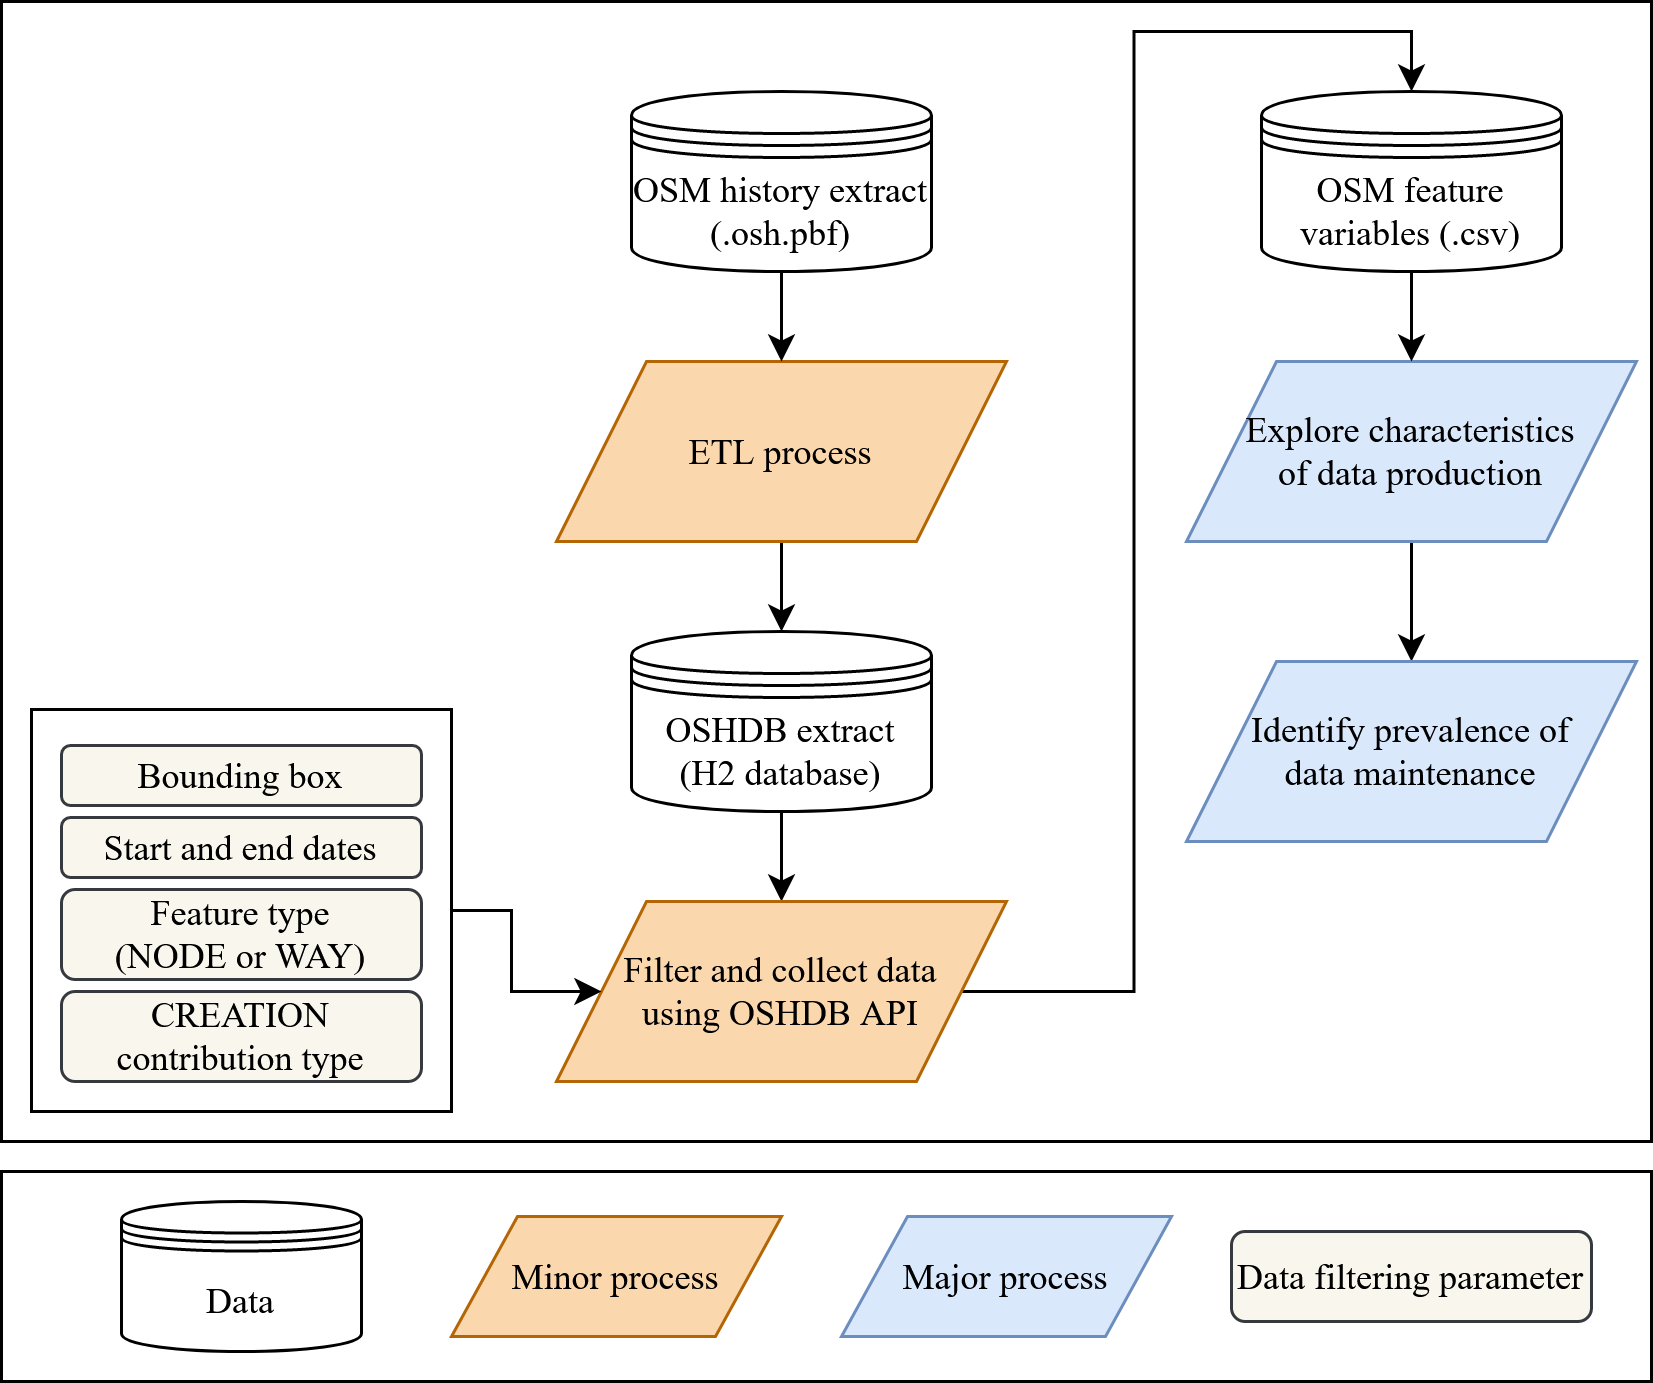
\includegraphics[width = \textwidth]{Images/Datapipeline.png} %this tells latex what graphics to include. 
    \caption{Summary of data processing pipeline.} % this prints the caption below the figure
    \label{fig:pipe} % this internally labels the figure for future referencing.
\end{figure}
%%%%%%%%%%%%%%%%%%%%%%%%%% 

To begin, each OSM history extract, in \textit{.osh.pbf} format, was converted to a local OSHDB instance, following the Extract, Transform, Load (ETL) process described in the OSHDB documentation.\footnote{\url{https://github.com/GIScience/oshdb/tree/master/oshdb-tool/etl}} This process loads the data from each extract into separate local H2 databases that are hosted locally. Each OSM entity is transformed into an OSH entity, a data format designed for use within the OSHDB framework. OSH features allow for more efficient storage of OSM data as they group together different versions of the same feature \parencite{raifer_oshdb_2019}. We note that some of the historical extracts were too large to be processed locally in this manner and so technical assistance in generating some extracts was provided by a researcher from the Heidelberg Institute for Geoinformatik Technology (HeiGIT) team. 

The OSHDB API \parencite{raifer_oshdb_2019} was then used to filter and process the historical data to obtain variables of interest.  Implemented in the Java programming language, this API allows for data filtering and aggregation based on the \textit{MapReduce} programming framework \parencite{raifer_oshdb_2019}. This framework is designed for use with large datasets and contains a \textit{map} function whereby data is filtered and sorted, followed by a \textit{reduce} function whereby data is summarized and returned as aggregated values \parencite{dean_mapreduce_2008}.

We collected data for each case study using the spatial and temporal extents specified in Table \ref{tab:cases}. Bounding boxes correspond to the smallest square area encompassing the city of interest (here with coordinates rounded to two decimal places for greater legibility). The start and end date for each of the humanitarian featuress was collected from the associated HOT project page.\footnote{\url{https://www.hotosm.org/projects/}} The start and end dates for the Heidelberg reference case were selected to cover a year-long period that was relatively early in the development of the map for this area, to be better compared against the humanitarian cases. 

%%%%%%%%%%%%%%%%%%%%%%%%%% TABLE 
\begin{table}
\centering
\caption{Details of the spatial and temporal extents used to filter data for each case study.}
\label{tab:cases}
\begin{tabular}{llll}
\toprule
Name                     & Start      & End        & Bounding box                 \\
\midrule
Heidelberg               & 2008-12-31 & 2009-12-31 & 8.57, 49.35, 8.79, 49.46     \\
Port au Prince         & 2010-01-12 & 2011-10-31 & -72.57, 18.34, -72.16, 18.63 \\
Bangui & 2013-03-23 & 2015-12-31 & 18.49, 4.32, 18.59, 4.49     \\
Tacloban           & 2013-11-10 & 2014-01-31 & 124.89, 11.18, 125.08, 11.34 \\
Kathmandu         & 2015-04-25 & 2015-12-31 & 85.27, 27.67, 85.38, 27.75  \\
\bottomrule
\end{tabular}
\end{table}
%%%%%%%%%%%%%%%%%%%%%%%%%%

For each of the case studies, we focused solely on the new data that was produced and disregarded any modifications to existing data. We also focused only on nodes and ways, given that these are the most common OSM features (disregarding relations), particularly in humanitarian mapping efforts. Thus using the OSHDB's \textit{stream()} functionality, we collected numerous variables from all OSM features that were created during this time, and all subsequent versions of these features that were created in the time following the mapping campaigns. For example, we collected the details about the OSM entity, \textit{Node X}, that was created during the mapping efforts in \textit{Case Study Y}. Here, \textit{Node X} would have a version \#1. By grouping together all versions of a given OSM entity within a parent OSH entity, the OSHDB data model also allowed us to collect information from all subsequent versions of \textit{Node X}. These subsequent versions reflect modifications that were made to \textit{Node X} after it was initially created, such as modifications to its geometry or tags. The variables collected for each OSM entity are summarized in Table \ref{tab:vars}. 

The information captured by these variables is diverse, encompassing numerical, spatial, temporal, and attributional information. We also note that, while most variables are highly structured, the information contained within the \textit{Tags} variable requires significant cleaning to be useful. Across all case studies, we have collected data from 308,147 OSM features. Due to the presence of multiple versions for some features, as described above, we note that not all of these features were created during times of each mapping campaign, as detailed in Table \ref{tab:cases}.

%%%%%%%%%%%%%%%%%%%%%%%%%% TABLE 
\begin{table}
\centering
\caption{Summary of variables collected from OSM entities.}
\label{tab:vars}
\begin{tabular}{lll}
\toprule
Variable       & Description                                                                                    & Data type   \\
\midrule
ID             & Unique identifier for OSM/OSH entity                                                           & Numeric     \\
User ID        & The user ID of the OSM contributor                                                             & Numeric     \\
Bounding box   & Bounding box for the OSH entity                                                                & Coordinates \\
Type           & Node or way                                                                                    & Text        \\
Version number & Version number for the OSM entity                                                              & Numeric     \\
Timestamp      & Time of feature creation                                                                        & Date/time   \\
Tags           & \begin{tabular}[c]{@{}l@{}}Tags and keys associated with the \\ OSM entity\end{tabular}        & Text        \\
Visibility     & \begin{tabular}[c]{@{}l@{}}Indicating whether or not the \\ node has been deleted\end{tabular} & Boolean  \\
\bottomrule
\end{tabular}
\end{table}
%%%%%%%%%%%%%%%%%%%%%%%%%%

\section{Exploring the characteristics of data production}
\label{sec-production}

This historical OSM data was then analyzed to understand the basic characteristics of data production for each mapping campaign. We performed numerous data processing steps to understand how the data was produced over time, where the data was produced over space, what sources contributed to data production, and what types of geographic features were produced. We also calculated numerous summary statistics for each case study to allow for quantitative comparison.

To understand the dynamics of data production over the duration of each mapping campaign, we aggregated all features by the day that they were produced. We calculated the total number of features produced and the unique number of contributors each day. We then calculated the relationship between these two variables, by day, using the Pearson correlation coefficient. 

We investigated the patterns of data production over space by visualizing the density of new features created within each study area. We created a dot-density map for each case study, as this effectively shows the geographic distribution of contributions in each study area \parencite{kimerling_dotting_2009}. We calculated the centroid from each feature's bounding box to create this point-based density visualization. 

We parsed the tags associated with each feature to understand the types of features that were mapped and their associated sources. While tagging conventions within the OSM community result in many standardized tags used across features, we conducted some basic text preprocessing to ensure that all text was normalized as much as possible, allowing for more accurate aggregation. We converted all characters to lowercase and removed non alpha-numeric characters. For each case study, we calculated the most frequently occurring tag keys (and not the associated values) to provide an indication of the types of features that were mapped. We also analyzed the values that are associated with the 'source' tag key across features as in \textcite{ahmouda_analyzing_2018}. While no longer a common tagging practice, the 'source' tag key has frequently been used within the OSM community as a way to indicate the information source behind a given contribution \parencite{noauthor_keysource_2020}. For example, features that were added to OSM by tracing Bing satellite imagery might be accompanied by the \texttt{source=Bing} key-value pair. We calculated the most frequently occurring source values for each case study to provide an indication of the common information sources (particularly to indicate remote vs local sources). 

In addition to the above analyses, we calculated various metrics to provide a basis for empirical comparison between case studies. These metrics are summarized in Table \ref{tab:metrics}. We calculate the total duration and size of study area, as well at the total number of unique features mapped and unique contributors. We also follow \textcite{dittus_mass_2017} in calculating the 'burstiness' of each case study and classifying each case study as an event or mission. The burstiness measure provides insight into the dynamics of data production and is particularly relevant in the context of humanitarian mapping, as data is often produced very quickly over time in response to a crisis \parencite{dittus_mass_2017}. 

%%%%%%%%%%%%%%%%%%%%%%%%%% TABLE 
\begin{table}
\centering
\caption{Metrics calculated to compare mapping activity across case studies.}
\label{tab:metrics}
\begin{tabular}{lll}
\toprule
Metric                      & Unit                               & Formula                                                                                                                  \\
\midrule
Duration                    & \(days\)                               & End date - start date                                                                                                    \\
Area                        & \(km^2\)             & Bounding box length * width                                                                                              \\
Total features created      & \(features\)                           & NA                                                                                                                       \\
Total unique contributors   & \(contributors\)                       & NA                                                                                                                       \\
Burstiness                  & \(days\)                               & \begin{tabular}[c]{@{}l@{}}Number of days until 50\% of all \\ contributions were made\end{tabular}                      \\
campaign style            & \textit{EVENT} or \textit{MISSION}                   & \begin{tabular}[c]{@{}l@{}}Event if burstiness \textless 60, or \\ Mission if burstiness \textgreater{}= 60\end{tabular} \\
\bottomrule
\end{tabular}
\end{table}
%%%%%%%%%%%%%%%%%%%%%%%%%%

Through the analysis described in this section, we hope to gain a greater understanding of the many dimensions of data production during humanitarian mapping campaigns. Comparison between the humanitarian case studies and the Heidelberg reference will allow us to identify points of difference and similarity between mapping in humanitarian vs non-humanitarian contexts. This understanding will provide valuable context that will allow for a more meaningful interpretation of the results of the following section on data maintenance following mapping campaigns.

\section{Identifying data maintenance activities}
\label{sec-maint}

We analyse the historical OSM data for each case study to understand the extent to which features are maintained following each case study mapping campaign. We define data maintenance in OSM to be the practice by which a given feature already existing within the database is updated, usually to reflect a real-world change that has taken place in the corresponding geographic feature.  For example, following a building renovation, the building's footprint may have changed, requiring updating to the geometry of the building's polygon in OSM. 
We operationalize this definition by following \textcite{quattrone_work_2017}, in considering data maintenance to have occurred any time that an OSM entity has a version greater than 1. This definition leads to a binary consideration of maintenance, in that a given feature is considered to be \textit{unmaintained} if it only has one version (indicating that it has not been modified since its initial creation), and is considered to have been \textit{maintained} if it has at least two versions (indicating that it has been modified at least once since its initial creation).  

In addition to this binary perspective, we also consider different degrees of maintenance across features by examining the total number of versions that they each contain. From this perspective, we are able to make a distinction not only between maintained and unmaintained features, but also between those that are more frequently maintained than others (ie. those that have a greater number of versions). While not explicitly considering the concept of data maintenance, \textcite{mooney_characteristics_2012} also analyze the version volume of OSM features, focusing specifically on highly-edited features (those with greater than 15 versions). Based on the distribution of version numbers across all features in our dataset, we create a classification of maintenance frequency, as detailed in Table \ref{tab:freq}. 

%%%%%%%%%%%%%%%%%%%%%%%%%%
\begin{table}[]
\centering
\caption{Classification scheme of maintenance frequency.}
\label{tab:freq}
\begin{tabular}{ll}
\toprule
Number of versions & Maintenance frequency \\
\midrule
1                  & Never                  \\
2                  & Once                  \\
3-10               & Moderate              \\
11-19              & Frequent              \\
20+                & Extreme               \\
\bottomrule
\end{tabular}
\end{table}
%%%%%%%%%%%%%%%%%%%%%%%%%%

We also quantified the temporal dimension of data maintenance, aiming to better understand \textit{when} maintenance occurs following a mapping campaign. To normalize across each of our case studies, we consider the four-year period following each of the mapping campaigns. For each year following the end of the campaign, we calculate a) the percentage of all features that have been maintained at least once, and b) the number of versions for all features. 

Additionally, we consider data maintenance from a more granular perspective by investigating the types of features that are maintained more frequently than others. We consider differences in maintenance between nodes and ways. We also identify the tags that are associated with the most and least frequently maintained features. 

Following these efforts to quantify data maintenance across each of our case studies, we interpret our results with respect to the findings from the previous section. We consider the results from Sections \ref{sec-production} and \ref{sec-maint} to develop informed hypotheses about how the modes of data production during humanitarian mapping campaigns may have an impact on the prevalence of data maintenance. Given the limited scope of this work, these hypothesis cannot be empirically validated, and so should be explored in greater depth in future work. 

\section{Ethical considerations}

Our analysis does not include the personal data from any individuals. 

TO DO
\chapter{Results}
\label{chapterlabel5}

In this chapter I offer the results of the analysis conducted in this research project. I will begin by providing background context for each of our selected case studies. I then summarize the characteristics of the data produced in each case study and provide an overview of the dynamics of data production over the duration of each mapping campaign. I will present results that demonstrate the prevalence of data maintenance following each campaign. 

\section{Case study context}

Prior to providing the empirical results of our analysis, I briefly address the humanitarian context in each of our case studies and their relevance to the humanitarian mapping community. The geographic location and spatial distribution of mapping activity for each case study can be seen in Figure \ref{fig:map}. Full-size versions of each inset map can be found in Appendix \ref{appendixlabel1}. 

%%%%%%%%%%%%%%%%%%%%%%%%%% Over time image 
\begin{figure} % opens the figure environment. the '[H]' forces the image to be Here
    \centering % puts the image in the horizontal centre of the page
    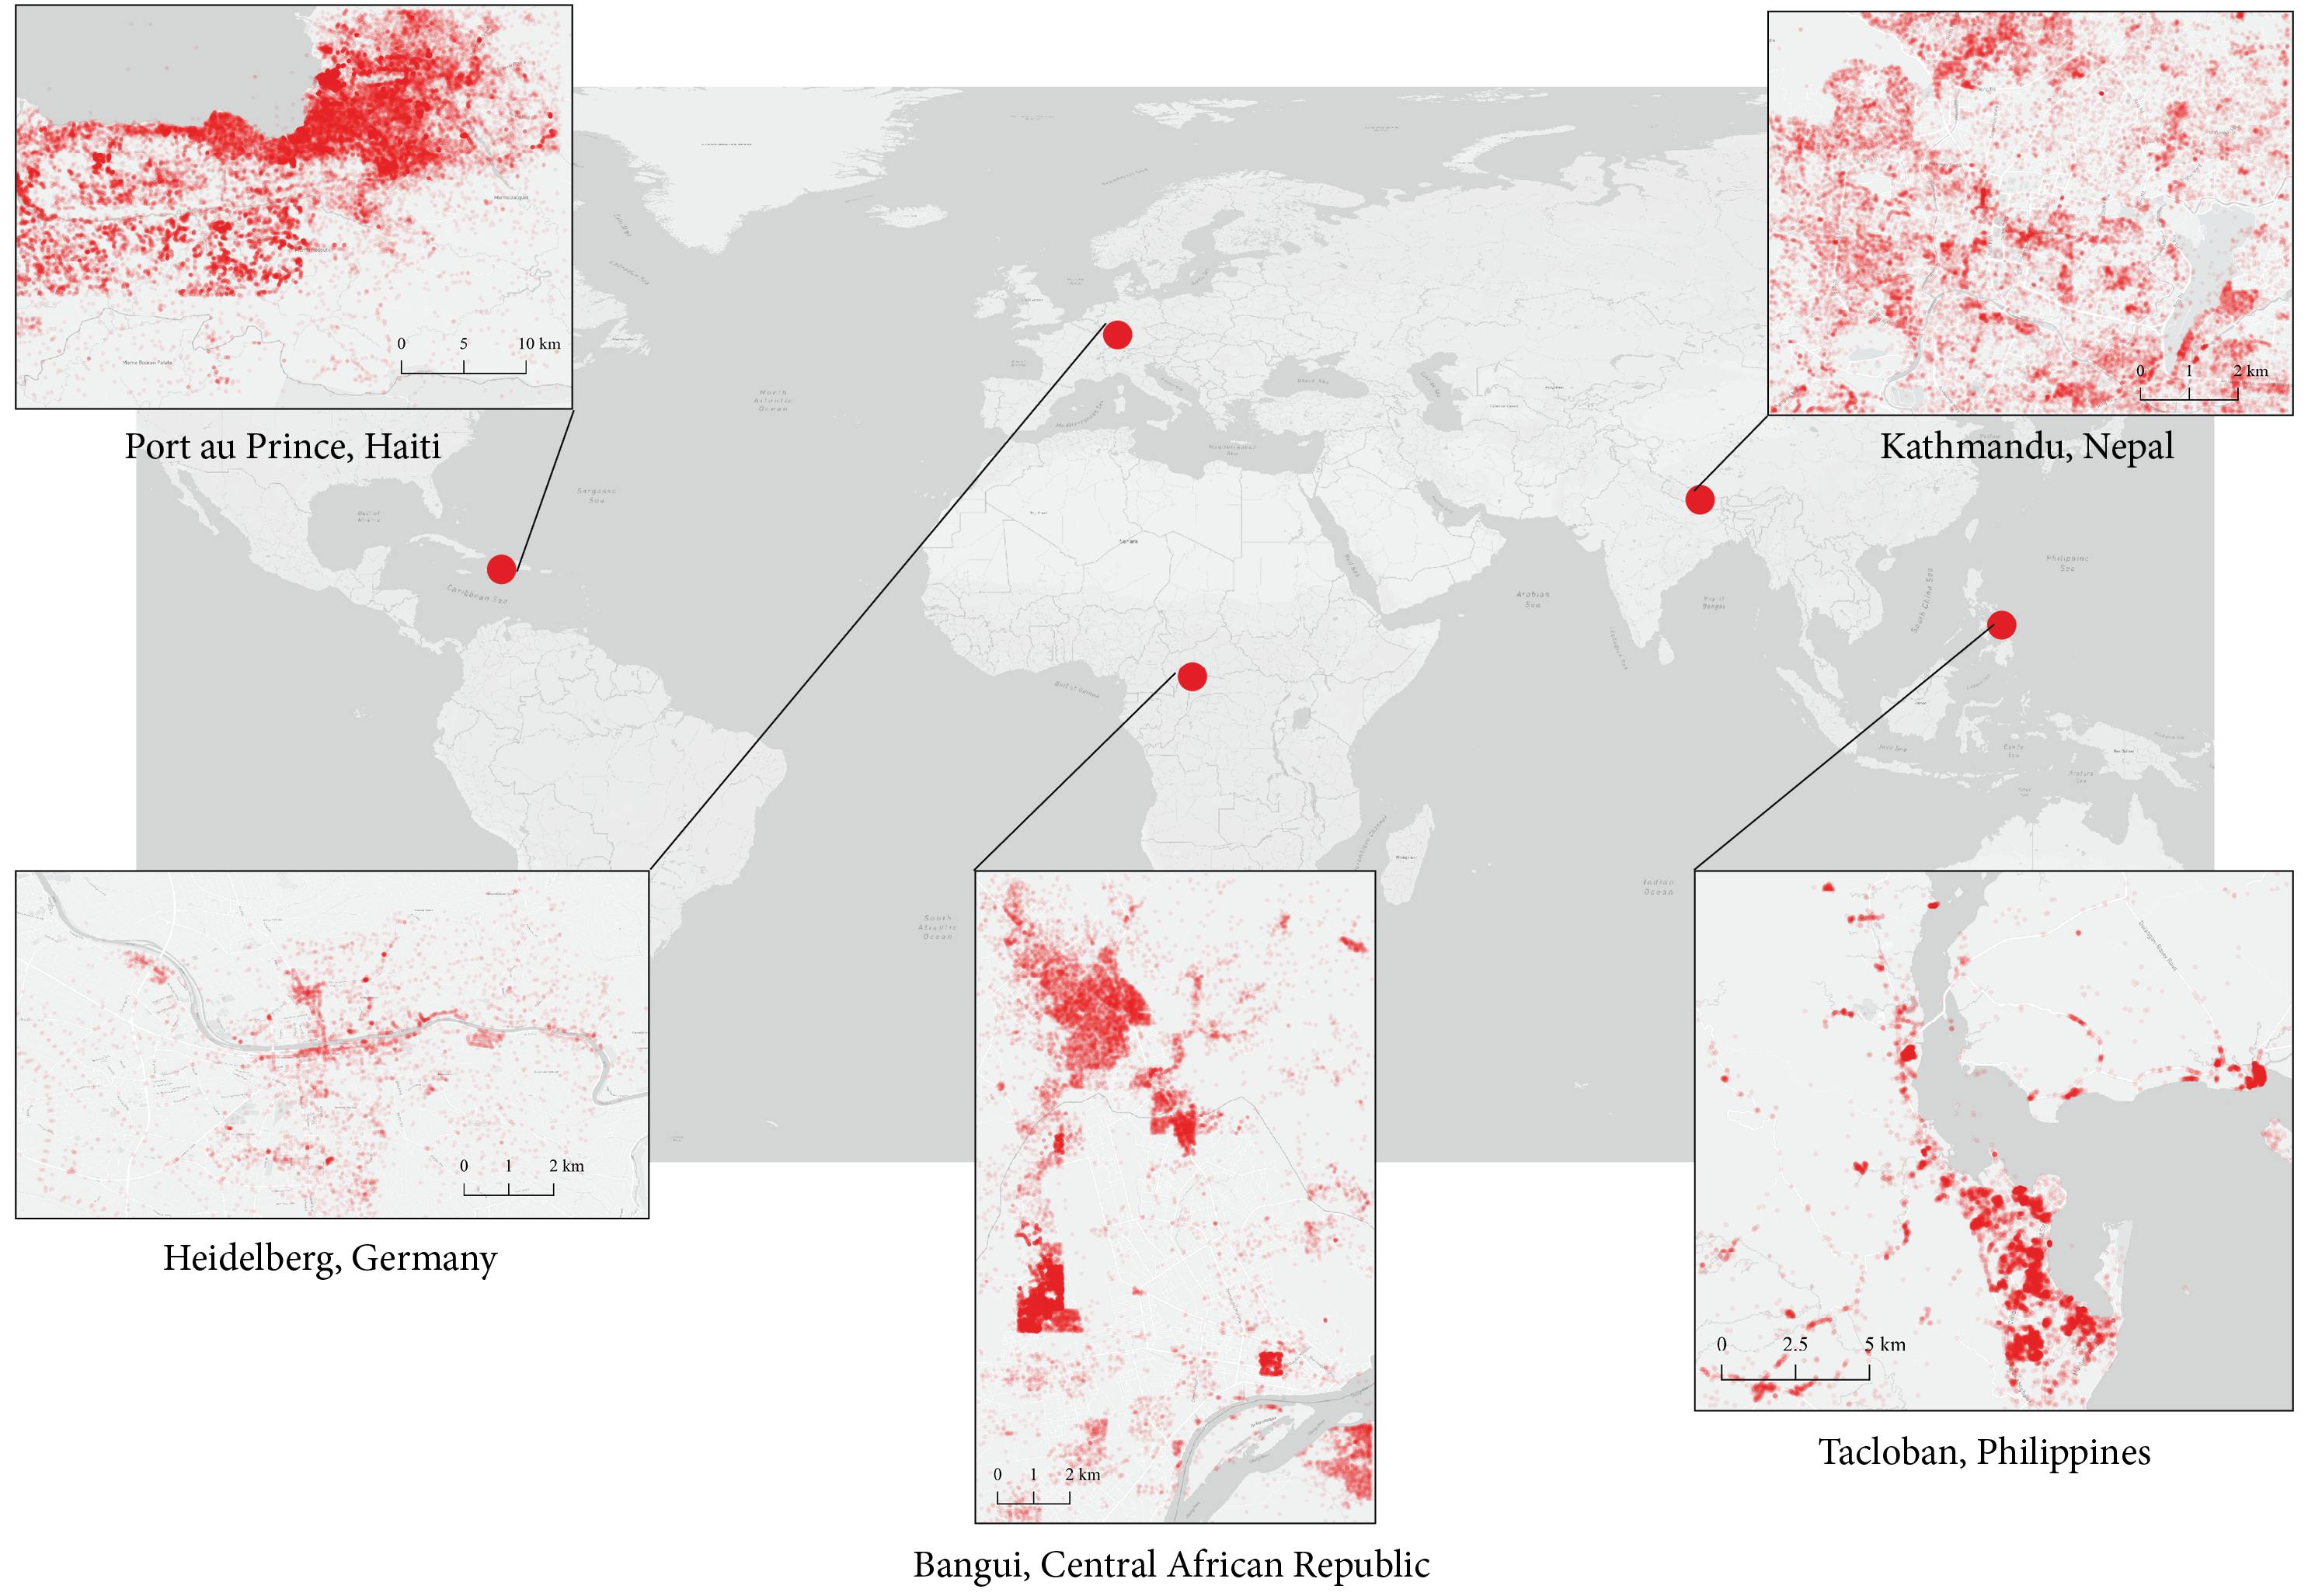
\includegraphics[width = \textwidth]{Images/sum_map.png} %this tells latex what graphics to include. 
    \caption[Map of case study locations and spatial distribution of features added.]{Map of case study locations and spatial distribution of features added. Greater intensity of colour corresponds to a greater density of features added to OSM during each mapping campaign.} % this prints the caption below the figure
    \label{fig:map} % this internally labels the figure for future referencing.
\end{figure}
%%%%%%%%%%%%%%%%%%%%%%%%%% 

\subsection{Port au Prince, Haiti}

Haiti experienced a magnitude 7.0 earthquake on January 12, 2010, which caused an estimated 300,000 deaths, and widespread building damage and population displacement \parencite{desroches_overview_2011}. The effects of the earthquake were further exacerbated by an outbreak of cholera in October 2010 that spread to informal settlements \parencite{human_rights_watch_world_2011}. It is estimated that this event has caused USD \$8.1bn damage \parencite{cavallo_estimating_2010}. Humanitarian mapping efforts in Haiti following this earthquake have been well researched and discussed in past academic literature \parencite{zook_volunteered_2010, soden_crowdsourced_2014, palen_success_2015, meier_crisis_2012}. This disaster has been described as a "catalyzing event" for many digitally-focused volunteer communities \parencite[p. 314]{soden_crowdsourced_2014}. Mapping efforts around this event also led to the formalization of the Humanitarian OpenStreetMap Team (HOT), the process of which is described in further detail by \textcite{soden_crowdsourced_2014}. Throughout their post-disaster efforts to raise awareness of the value of OSM and mobilize a community of mappers, one of HOT's primary goals was to "embed" OSM within the local community and further local ownership of this data. This effort was intended to allow for the long-term use of OSM data beyond this humanitarian response \parencite{soden_crowdsourced_2014}. As shown by Figure \ref{fig:map}, the features mapped within this study area are largely clustered around the coast of Port au Prince. 

\subsection{Tacloban, Philippines}

The Philippines was greatly impacted by a tropical cyclone, Typhoon Haiyan (or Typhoon Yolanda), on November 8, 2013. This typhoon is said to be one of the strongest ever recorded \parencite{lum_typhoon_2014}. USAID estimates that this disaster has caused over 6,000 deaths and the destruction or damage of over 1 million homes \parencite{noauthor_typhoon_2014}. The city of Tacloban was one of the areas that faced greatest impact and was thus where much relief effort was focused \parencite{lum_typhoon_2014}, as shown by the clustering of features on the inset map in Figure \ref{fig:map}. Following this crisis, mapping efforts in OSM were coordinated by HOT, with high-volume, remote mapping efforts organized by the newly developed Tasking Manager \parencite{openstreetmap_wiki_wikiproject_2018}. \textcite{palen_success_2015} note that the mapping efforts in the Philippines were facilitated by these new tools for technical collaboration, which incorporated lessons learned from previous humanitarian mapping efforts, such as in Haiti. Details from the OSM Wiki page indicate that most mapping efforts were focused on buildings, roads, and infrastructure damage \parencite{openstreetmap_wiki_wikiproject_2018}.

\subsection{Kathmandu, Nepal}

Nepal was hit with a magnitude 7.6 earthquake on April 25th, centered approximated 76 km northwest of Kathmandu, which was followed by over 300 aftershocks of over 4.0 magnitude \parencite{noauthor_nepal_2015}. It is estimated that over 9,000 people died in these disasters and over half a million homes were destroyed or damaged \parencite{noauthor_nepal_2015}. The major earthquake and its aftershocks caused further disasters such as landslides and avalanches, and exacerbated vulnerabilities to flooding in many areas \parencite{noauthor_nepal_2015}. As is described by \textcite{soden_infrastructure_2016} this crisis can be viewed as a turning point in the history of post-disaster mapping in the OSM community. Whereas in the Haiti case where HOT needed to conduct notable outreach to spread awareness of the applicability of OSM data, interviews with GIS practitioners in the field found that up-to-date OSM data came to be an "expected resource" in Nepal \parencite[p. 2801]{soden_infrastructure_2016}. Figure \ref{fig:map} shows how the mapping activity is decentralized throughout our study area of Kathmandu.

\subsection{Bangui, Central African Republic}

Violence and instability in CAR mounted in March 2013 when the Seleka rebel group seized the capital city, Bangui \parencite{global_conflict_tracker_violence_2020}. This event launched a humanitarian mapping campaign that aimed to provide baseline geospatial data for the country \parencite{openstreetmap_wiki_wikiproject_2020}. Mapping the country's road network was a priority of this campaign, as well as mapping affected cities and towns, as identified by local humanitarian stakeholders \parencite{openstreetmap_wiki_wikiproject_2020}. The features mapped within our study area in Bangui are clustered within the periphery of the area, as shown in Figure \ref{fig:map}. UNICEF data for health facilities, water points, and schools was also imported as part of this campaign \parencite{openstreetmap_wiki_wikiproject_2020}.

\subsection{Heidelberg, Germany}

Heidelberg serves as our reference case study, allowing us to compare humanitarian mapping activities with those from a part of the map that has been established as high quality (researched by \textcite{arsanjani_assessing_2013} and previously applied as a reference case study by \textcite{anderson_crowd_2018}). While I generalize and refer to all of our case studies as "mapping campaigns", I acknowledge that this Heidelberg case does not refer to a distinct campaign, as with our other humanitarian case studies. Figure \ref{fig:map} shows how the features mapped in this case study are distributed around the centre of our study area.

\section{Characteristics of OSM data production}

In this section, I provide details of the data that was produced in each of our case studies.

%%%%%%%%%%%%%%%%%%%%%%%%%% TABLE - summary
\begin{table}[H]
\centering
\caption{Summary statistics for data produced in each case study.}
\label{tab:summary}
\begin{tabular}{lllllll} 
\toprule
Case Study     & \begin{tabular}[c]{@{}l@{}}Duration\\$Days$\end{tabular} & \begin{tabular}[c]{@{}l@{}}Area\\$km^2$\end{tabular} & \begin{tabular}[c]{@{}l@{}}Unique \\Contributors\end{tabular} & \begin{tabular}[c]{@{}l@{}}Features\\Created\end{tabular} & Burst & Style    \\ 
\midrule
Port au Prince & 658                                                      & 1397                                                 & 313                                                           & 31962                                                     & 17    & event    \\
Tacloban       & 82                                                       & 356                                                  & 199                                                           & 19801                                                     & 1     & event    \\
Kathmandu      & 250                                                      & 98                                                   & 881                                                           & 37587                                                     & 5     & event    \\
Bangui         & 1012                                                     & 203                                                  & 170                                                           & 36788                                                     & 164   & mission  \\
Heidelberg     & 365                                                      & 192                                                  & 108                                                           & 3786                                                      & 146   & mission  \\
\bottomrule
\end{tabular}
\end{table}
%%%%%%%%%%%%%%%%%%%%%%%%%% 

Table \ref{tab:summary} provides a basic summary of the data produced in each case study. I see that each case study covers varying temporal and spatial extents. The mapping campaign in Bangui, for example, is over ten times longer than that in Tacloban. The mapping campaign in Port au Prince covers an area that is nearly 15 times larger than that in Kathmandu. Despite these differences, all humanitarian mapping campaigns have produced volumes of data that are of the same order of magnitude (approximately 20,000 to 40,000 new features created). The reference case study in Heidelberg has produced notably less data. The case study in Kathmandu stands out when considering the number of unique contributors (nearly three-times the case study with the next largest number), and the density of contributors over space. The burstiness value, which corresponds to the number of days until 50\% of all the data from the campaign has been created, for each case study results in the ‘style’ classification \parencite{dittus_mass_2017}. Both Bangui and Heidelberg are classified as "missions", while Port au Prince, Tacloban, and Kathmandu are "events". 

%%%%%%%%%%%%%%%%%%%%%%%%%% Over time image 
\begin{figure} % opens the figure environment. the '[H]' forces the image to be Here
    \centering % puts the image in the horizontal centre of the page
    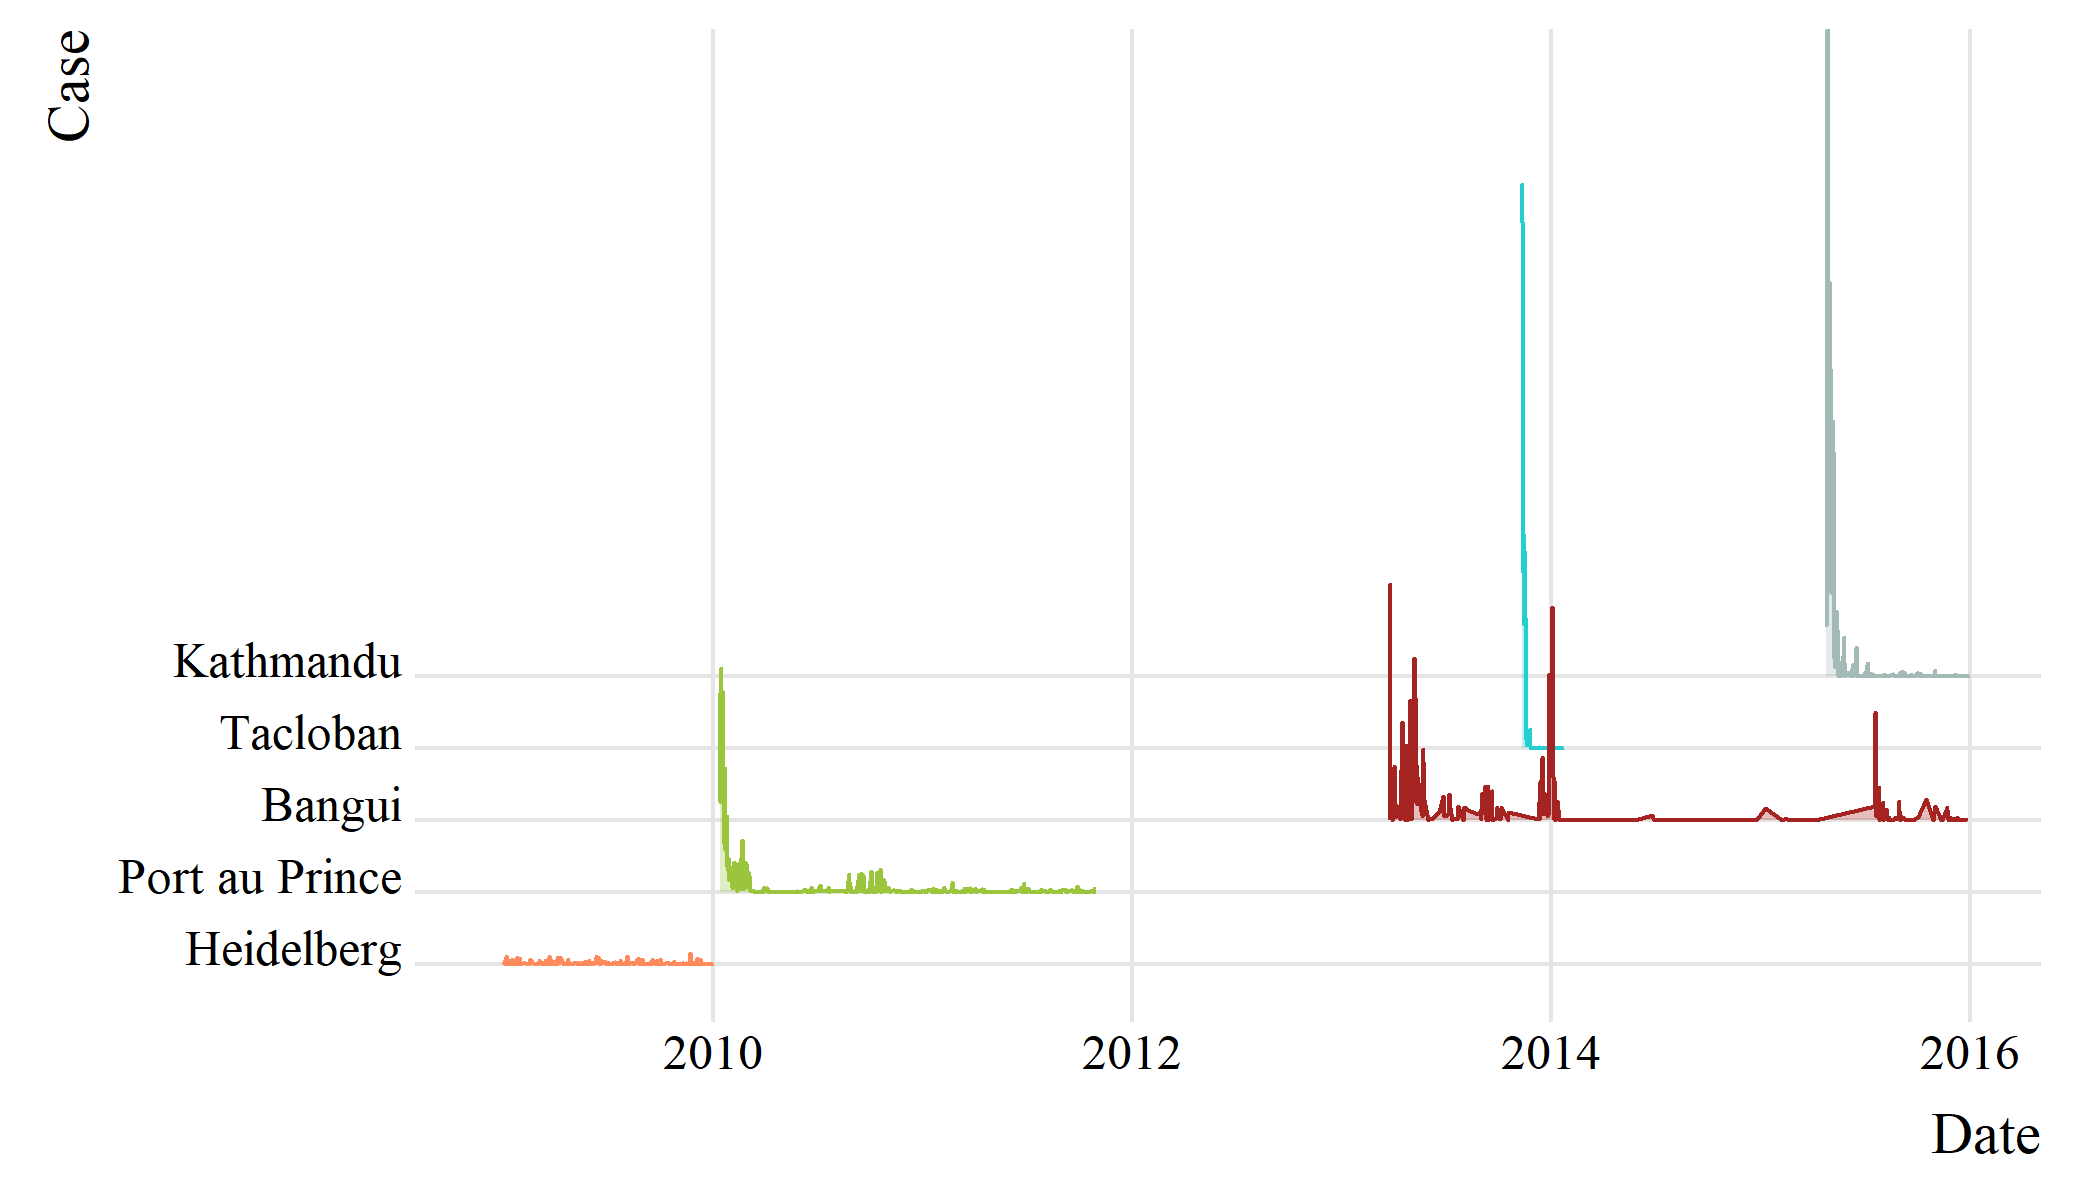
\includegraphics[width = \textwidth]{Images/overtime.png} %this tells latex what graphics to include. 
    \caption[Daily volume of OSM contributions throughout duration of each mapping campaign.]{Daily volume of OSM contributions throughout duration of each mapping campaign. The implied z-axis indicates the relative daily contribution volume.} % this prints the caption below the figure
    \label{fig:time} % this internally labels the figure for future referencing.
\end{figure}
%%%%%%%%%%%%%%%%%%%%%%%%%% 

The dynamics of contributing patterns for each case study are further demonstrated in Figure \ref{fig:time}, which shows the daily magnitude of contributions for each mapping campaign. The campaigns in Tacloban, Port au Prince, and Kathmandu exhibit the characteristics of event-style campaigns, as described by \textcite{dittus_mass_2017}, whereby mapping activity is front-loaded and decays quickly after the beginning of the campaign. The magnitude of early mapping efforts in Tacloban, Kathmandu, and Port au Prince, shown by the burstiness values from Table \ref{tab:summary} and the size of the peaks in Figure \ref{fig:time}, set these cases apart from others. The mapping in Bangui and the Heidelberg reference show a pattern where activity is more evenly sustained over a longer period of time. 

Further differences between the two mapping campaign styles are shown in Figure \ref{fig:scatter}, where I see that the ‘event-style’ campaigns have a stronger relationship between the number of daily contributors and contributions.  In all cases, however, the relationship between daily contributor volume and daily contribution volume is statistically significant. Heidelberg and Bangui, the two ‘mission-style’ campaigns, have a notably shorter range of daily unique contributors (no more than 10 in a day), while campaigns such as that in Kathmandu have reached over 150 unique contributors in a day. 

%%%%%%%%%%%%%%%%%%%%%%%%%% Scatter image
\begin{figure} % opens the figure environment. the '[H]' forces the image to be Here
    \centering % puts the image in the horizontal centre of the page
    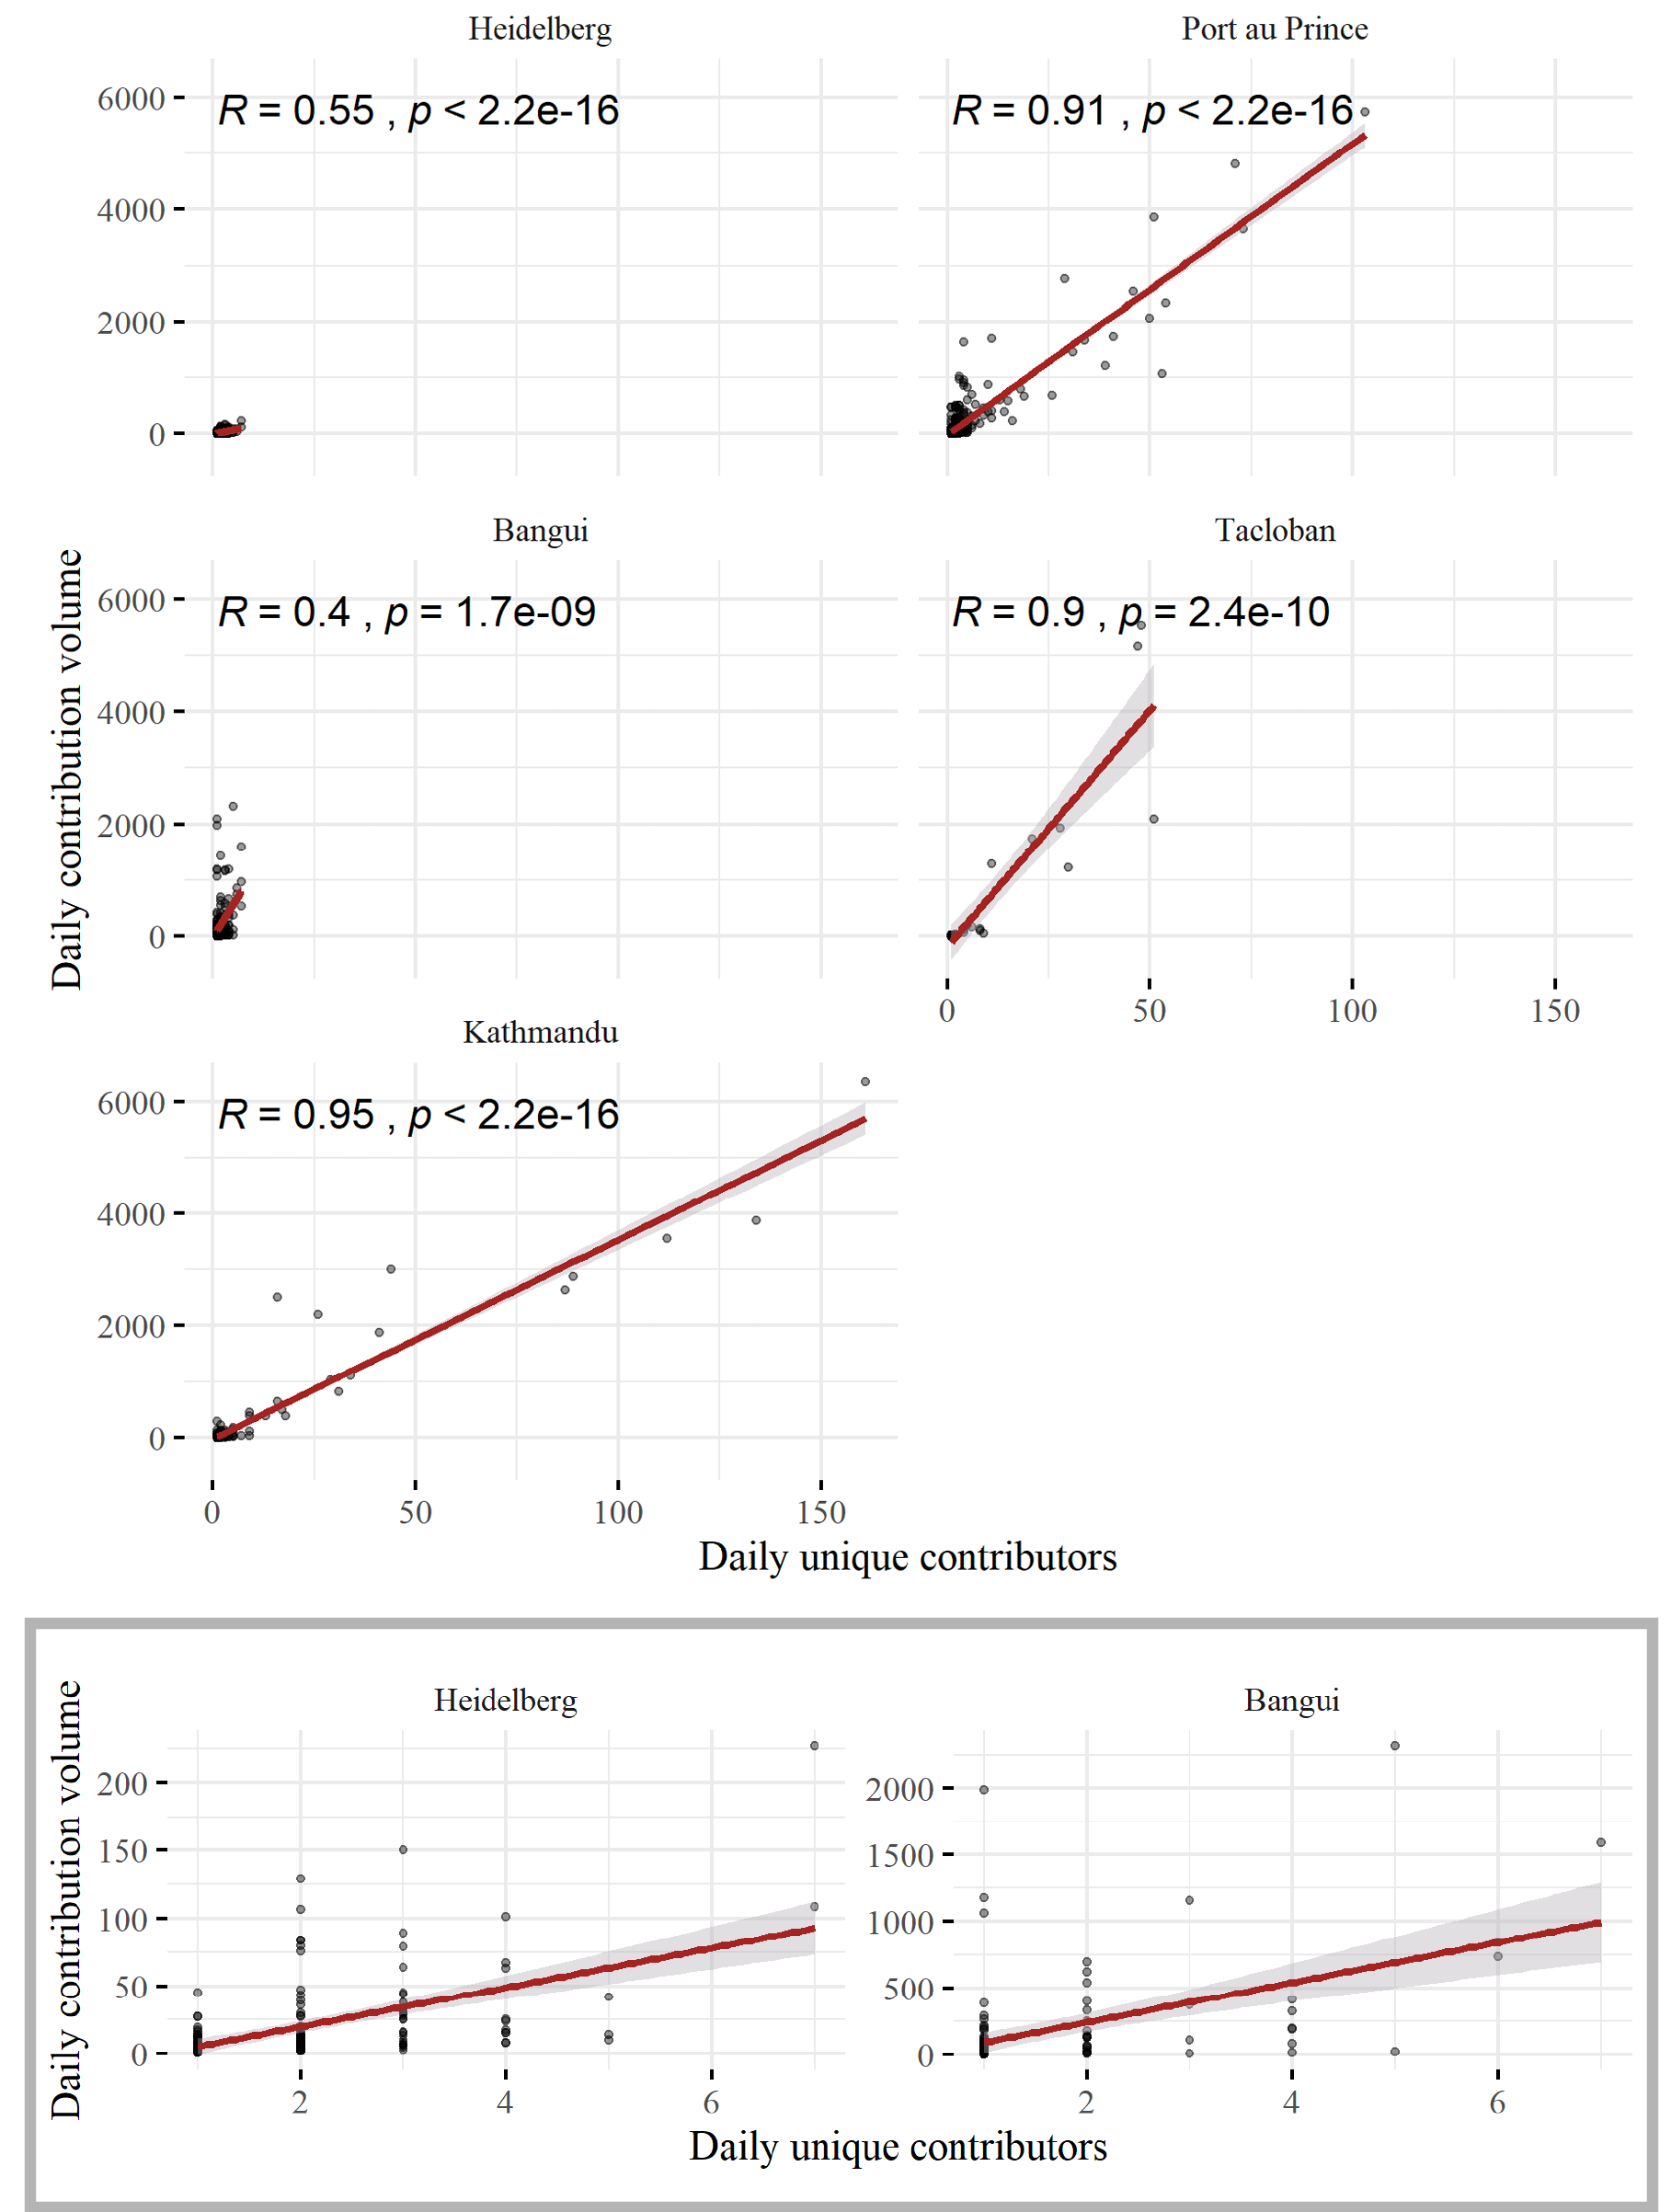
\includegraphics[width = \textwidth]{Images/scatter_inset.png} %this tells latex what graphics to include. 
    \caption[Scatterplots of daily unique contributors against daily contribution volume.]{Scatterplots of daily unique contributors against daily contribution volume (in number of contributions) for each mapping campaign. Includes inset of Heidelberg and Bangui with rescaled axes.} % this prints the caption below the figure
    \label{fig:scatter} % this internally labels the figure for future referencing.
\end{figure}
%%%%%%%%%%%%%%%%%%%%%%%%%% 

Both Figures \ref{fig:time} and \ref{fig:scatter} show a clear difference in the daily volume of data contributed between the Heidelberg reference and the humanitarian campaigns.  Daily contribution volume in Heidelberg during this time barely exceed 100 new features, while humanitarian campaigns such as those in Tacloban and Kathmandu reach over 4,000 and 6,000 new features in a day, respectively, at their peaks. 

Table \ref{tab:tags}, below, provides insight into the type of data that is contributed in each mapping campaign. I see similarities across all cases as the \texttt{building}, \texttt{highway}, and \texttt{source} tags are frequently occurring in each. The humanitarian campaigns show crisis-specific tags, such as \texttt{typhoon:damage} and \texttt{damage:event}.  

Table \ref{tab:sources} provides insight into the data sources for each mapping campaign. For the humanitarian cases, I see that a notable proportion of the data was generated from satellite imagery (eg. Bing or Worldview), suggesting that many of the contributors are remotely located. Very little of the Heidelberg data has been tagged with a source, however none of the sources listed are from satellite imagery, so I can perhaps infer that much of this data was added by local contributors. 

%%%%%%%%%%%%%%%%%%%%%%%%%% TABLE - tags 
\begin{table}[H]
\centering
\caption[Frequently occurring tag keys.]{Top five most frequently occurring tag keys across each case study. Keys highlighted in grey appear across at least 4/5 case studies.}
\label{tab:tags}
\begin{tabular}{@{} llll @{}} 
\toprule
Port au Prince                               &                  & Tacloban                                     &                   \\ 
\midrule
\textit{key}                                 & \textit{percent} & \textit{key}                                 & \textit{percent}  \\
{\cellcolor[rgb]{0.875,0.875,0.875}}source   & \Chart{0.76}             & {\cellcolor[rgb]{0.875,0.875,0.875}}building & \Chart{0.89}              \\
{\cellcolor[rgb]{0.875,0.875,0.875}}highway  & \Chart{0.33}             & {\cellcolor[rgb]{0.875,0.875,0.875}}source   & \Chart{0.27}              \\
{\cellcolor[rgb]{0.875,0.875,0.875}}building & \Chart{0.29}             & typhoon:damage                               & \Chart{0.11}                \\
attribute\_source\_date                      & \Chart{0.17}             & {\cellcolor[rgb]{0.875,0.875,0.875}}highway  & \Chart{0.27}               \\
name                                         & \Chart{0.11}             & typhoon:damaged                              & \Chart{0.15}               \\ 
\toprule
Bangui                                       &                  & Kathmandu                                    &                   \\ 
\midrule
\textit{key}                                 & \textit{percent} & \textit{key}                                 & \textit{percent}  \\
{\cellcolor[rgb]{0.875,0.875,0.875}}building & \Chart{0.58}             & {\cellcolor[rgb]{0.875,0.875,0.875}}building & \Chart{0.74}              \\
{\cellcolor[rgb]{0.875,0.875,0.875}}source   & \Chart{0.35}               & {\cellcolor[rgb]{0.875,0.875,0.875}}source   & \Chart{0.24}              \\
{\cellcolor[rgb]{0.875,0.875,0.875}}highway  & \Chart{0.11}             & idp:camp\_site                               & \Chart{0.14}              \\
source:date                                  & \Chart{0.06}              & damage:event                                 & \Chart{0.13}              \\
project:eurosha\_2012                        & \Chart{0.06}              & {\cellcolor[rgb]{0.875,0.875,0.875}}highway  & \Chart{0.04}               \\ 
\toprule
Heidelberg                                   &                  &                                              &                   \\ 
\midrule
\textit{key}                                 & \textit{percent} &                                              &                   \\
{\cellcolor[rgb]{0.875,0.875,0.875}}highway  & \Chart{0.46}             &                                              &                   \\
name                                         & \Chart{0.23}               &                                              &                   \\
tracktype                                    & \Chart{0.14}             &                                              &                   \\
created\_by                                  & \Chart{0.13}             &                                              &                   \\
amenity                                      & \Chart{0.10}              &                                              &     \\
\bottomrule
\end{tabular}
\end{table}
%%%%%%%%%%%%%%%%%%%%%%%%%%

%%%%%%%%%%%%%%%%%%%%%%%%%% TABLE - sources
\begin{table}[H]
\centering
\caption[Frequently occurring sources for data from each case study.]{Top five most frequently occurring source tag values for data from each case study. }
\label{tab:sources}
\begin{tabular}{llll} 
\toprule
Port au Prince                                                                                                                    &                  & Tacloban                                                                                    &                   \\ 
\midrule
\textit{source}                                                                                                                   & \textit{percent} & \textit{source}                                                                             & \textit{percent}  \\
geoeye                                                                                                                            & \Chart{0.230}            & bing                                                                                        & \Chart{0.131}              \\
google; 2010-01-21                                                                                                                & \Chart{0.150}            & \begin{tabular}[c]{@{}l@{}}Worldview-2; \\digitalglobe;\\nextview;\\2013/11/09\end{tabular} & \Chart{0.100}              \\
yahoo                                                                                                                             & \Chart{0.043}             & bing; 2010-11                                                                               & \Chart{0.018}              \\
NA                                                                                                                                & \Chart{0.042}             & gsi/kiban 2500; naro                                                                        & \Chart{0.004}              \\
google 2010-01-17                                                                                                                 & \Chart{0.033}             & \begin{tabular}[c]{@{}l@{}}hot task 355 \\image (arcgis)\end{tabular}                       & \Chart{0.021}              \\ 
\toprule
Bangui                                                                                                                            &                  & Kathmandu                                                                                   &                   \\ 
\midrule
\textit{source}                                                                                                                   & \textit{percent} & \textit{source}                                                                             & \textit{percent}  \\
bing                                                                                                                              & \Chart{0.186}            & \begin{tabular}[c]{@{}l@{}}pleiades 2015-04-27;\\cnes;airbus ds\end{tabular}                & \Chart{0.135}              \\
bing 2012                                                                                                                         & \Chart{0.132}            & nextview                                                                                    & \Chart{0.079}              \\
worldview1                                                                                                                        & \Chart{0.015}             & bing                                                                                        & \Chart{0.014}              \\
bing et hotosm                                                                                                                    & \Chart{0.012}             & gsimaps/std                                                                                 & \Chart{0.005}              \\
NA                                                                                                                                & \Chart{0.003}             & bing imagery                                                                                & \Chart{0.001}              \\ 
\toprule
Heidelberg                                                                                                                        &                  &                                                                                             &                   \\ 
\midrule
\textit{source}                                                                                                                   & \textit{percent} &                                                                                             &                   \\
survey                                                                                                                            & \Chart{0.017}             &                                                                                             &                   \\
\begin{tabular}[c]{@{}l@{}}http://wiki.openstreetmap\\.org/wiki/import/catalogue\\/kreisgrenzen\_deutschland\\\_2005\end{tabular} & \Chart{0.002}             &                                                                                             &                   \\
gps                                                                                                                               & \Chart{0.001}             &                                                                                             &                   \\
estimation                                                                                                                        & \Chart{0.001}             &                                                                                             &                   \\
rectified\_map:837                                                                                                                & \Chart{0.001}              &                                                                                             &       \\
\bottomrule
\end{tabular}
\end{table}
%%%%%%%%%%%%%%%%%%%%%%%%%% 

\section{Prevalence of data maintenance}

Following a review of the characteristics of data production across case studies, I now present results that provide insight into the trajectory of this data over time. Specifically, these results indicate the prevalence of data maintenance efforts in the years following each mapping campaign. 

%%%%%%%%%%%%%%%%%%%%%%%%%% Tot maintenance
\begin{figure} % opens the figure environment. the '[H]' forces the image to be Here
    \centering % puts the image in the horizontal centre of the page
    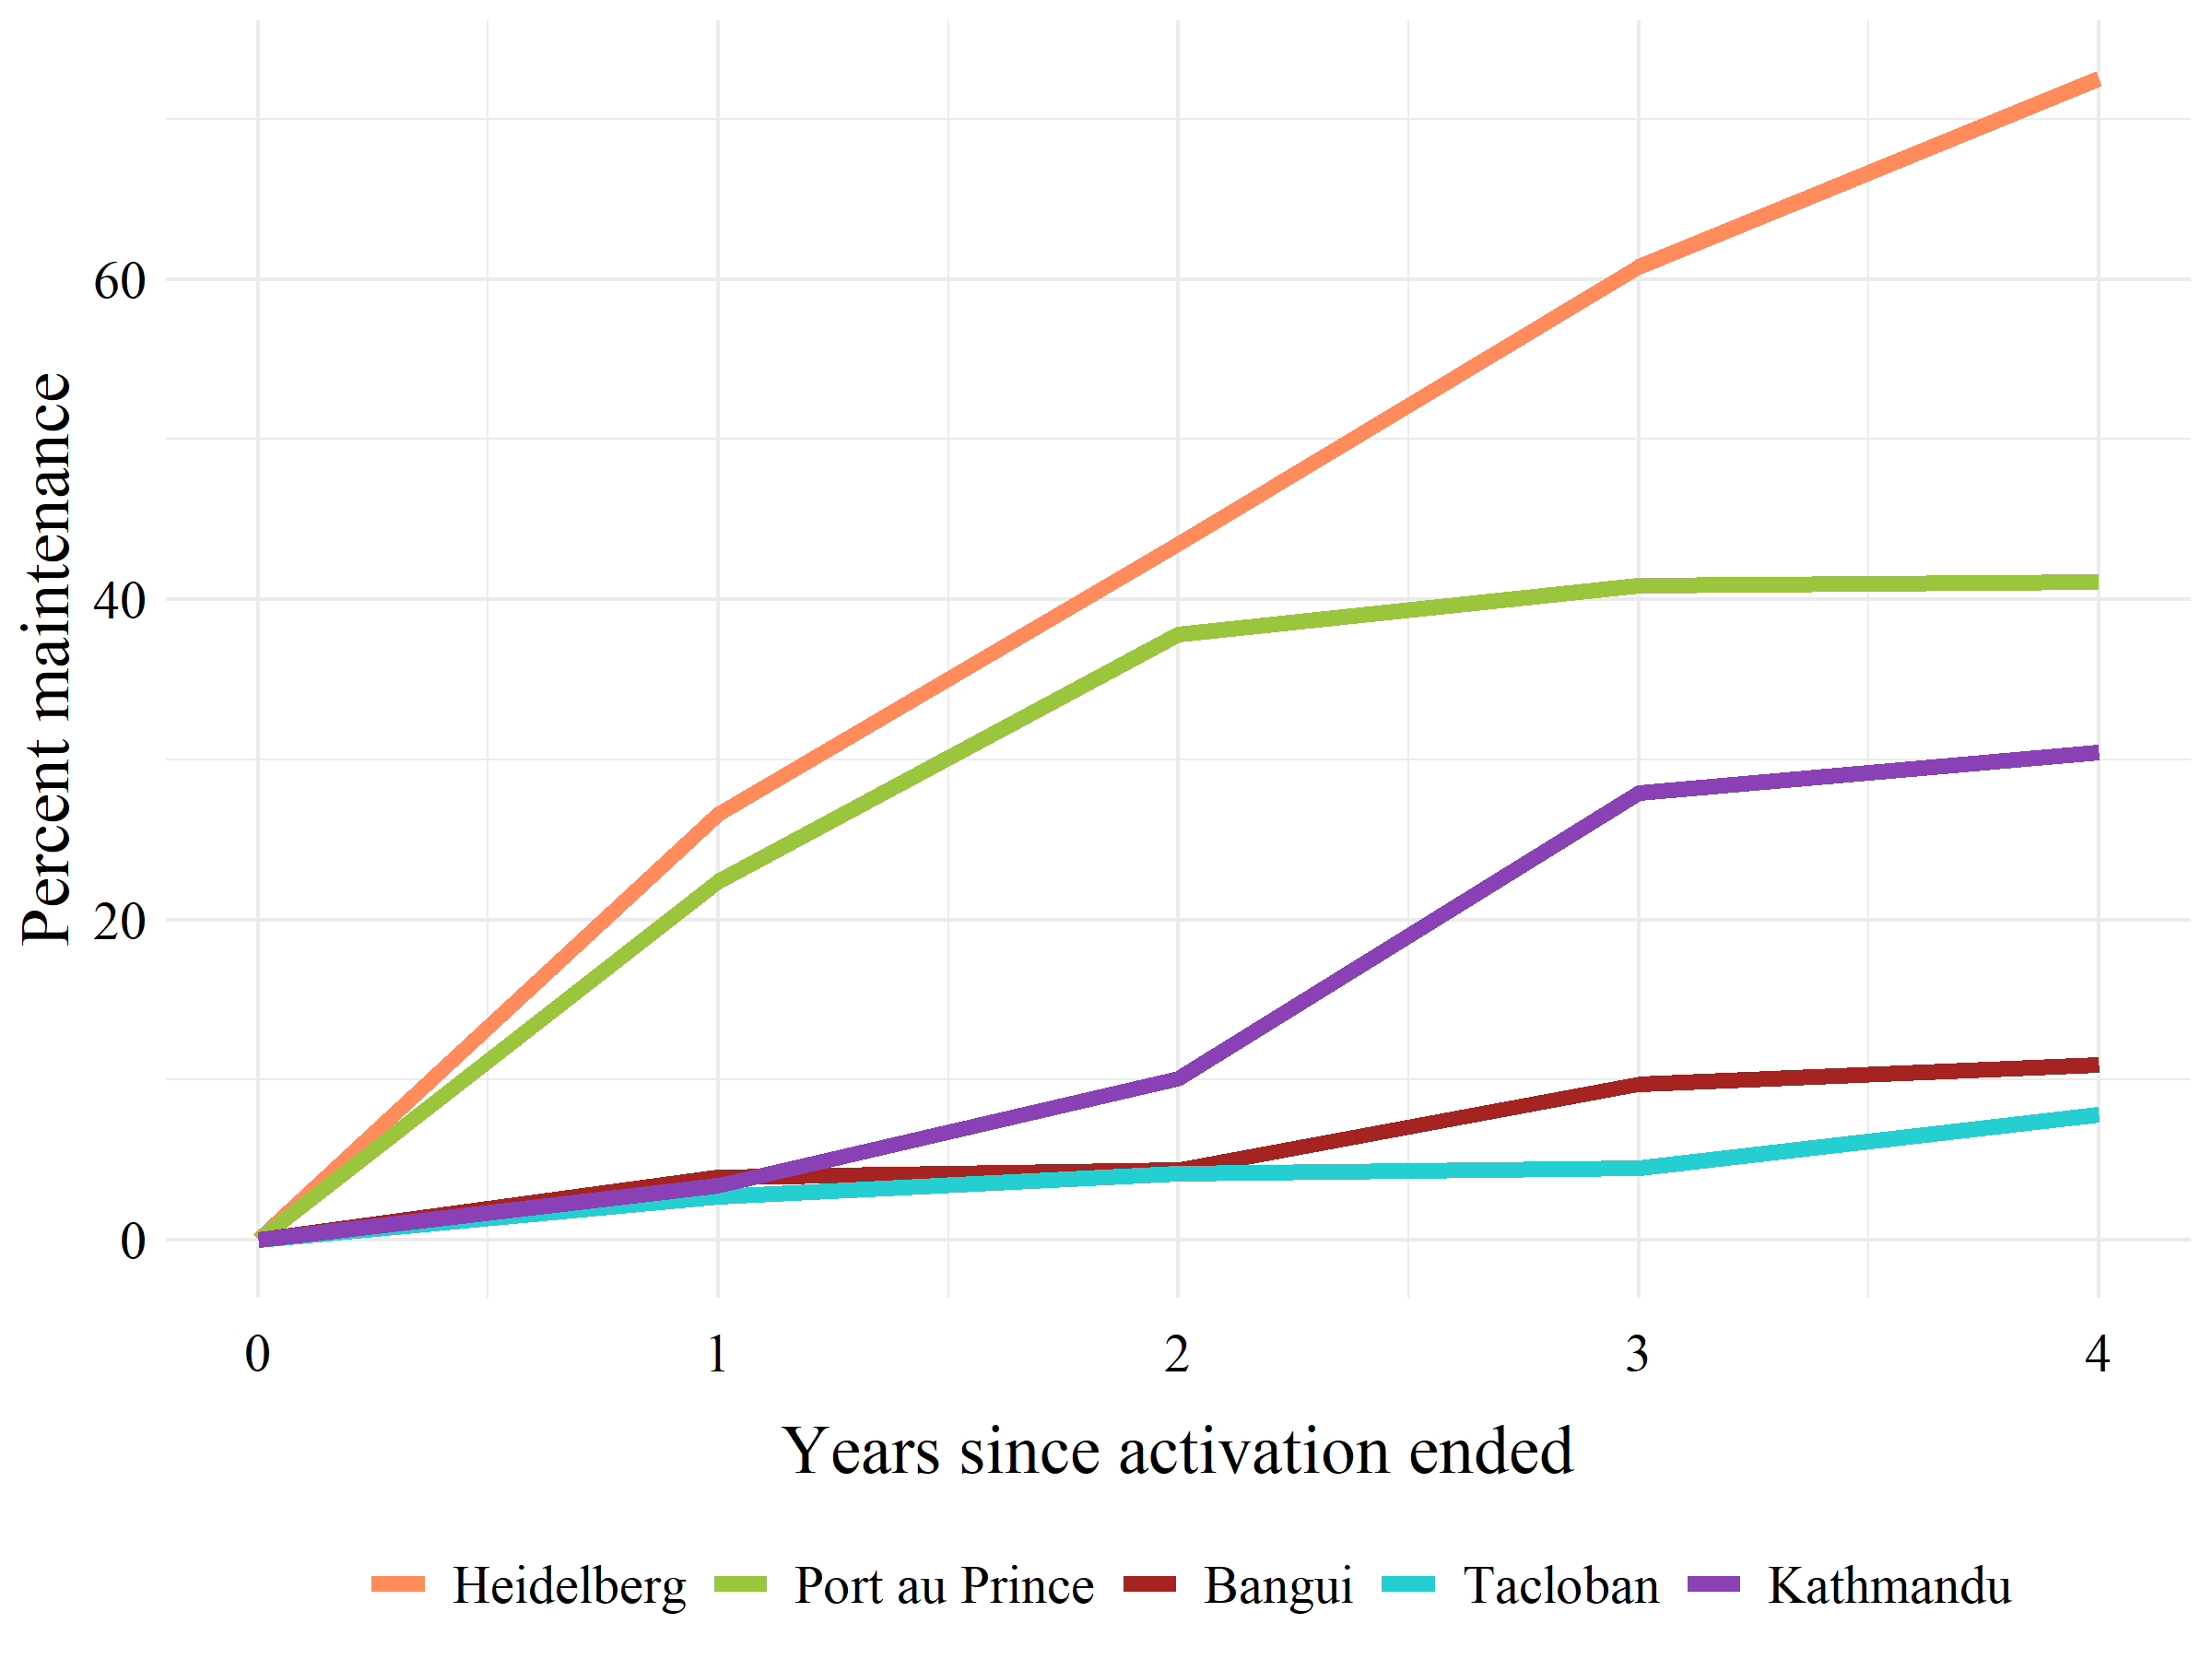
\includegraphics[width = \textwidth]{Images/totmaint.png} %this tells latex what graphics to include. 
    \caption[Percent of total maintained data over time.]{Cumulative percentage of maintained data (deleted or modified at least once) in years following end of mapping campaign} % this prints the caption below the figure
    \label{fig:tot} % this internally labels the figure for future referencing.
\end{figure}
%%%%%%%%%%%%%%%%%%%%%%%%%% 

Figure \ref{fig:tot}, above, provides an initial look at the prevalence of data maintenance in each case study. This figure shows the cumulative percentage of features, created during the mapping campaign period, that have been modified at least once in the years after the campaign has ended. I note that this and all subsequent figures include entity deletion within the definition of maintenance. 

I see that the reference case study, Heidelberg, has a significantly higher prevalence of data maintenance, as over 70\% of this data has been modified or deleted in the four years after it was originally created. Among the humanitarian case studies, the Port au Prince and Kathmandu campaigns stand out for both reaching above 30\% maintenance by the end of this four-year period. The other humanitarian case studies in Tacloban and Bangui only reach approximately 10\% maintenance during this time. Figure \ref{fig:tot} also shows how the rate of maintenance in Heidelberg appears to be approximately consistent during this time period, while maintenance efforts in the humanitarian case studies have plateaued in the fourth year after the campaign has ended. Maintenance efforts in Kathmandu increased notably in the third year after the campaign ended.

%%%%%%%%%%%%%%%%%%%%%%%%%% Distribution of maintenance
\begin{figure} % opens the figure environment. the '[H]' forces the image to be Here
    \centering % puts the image in the horizontal centre of the page
    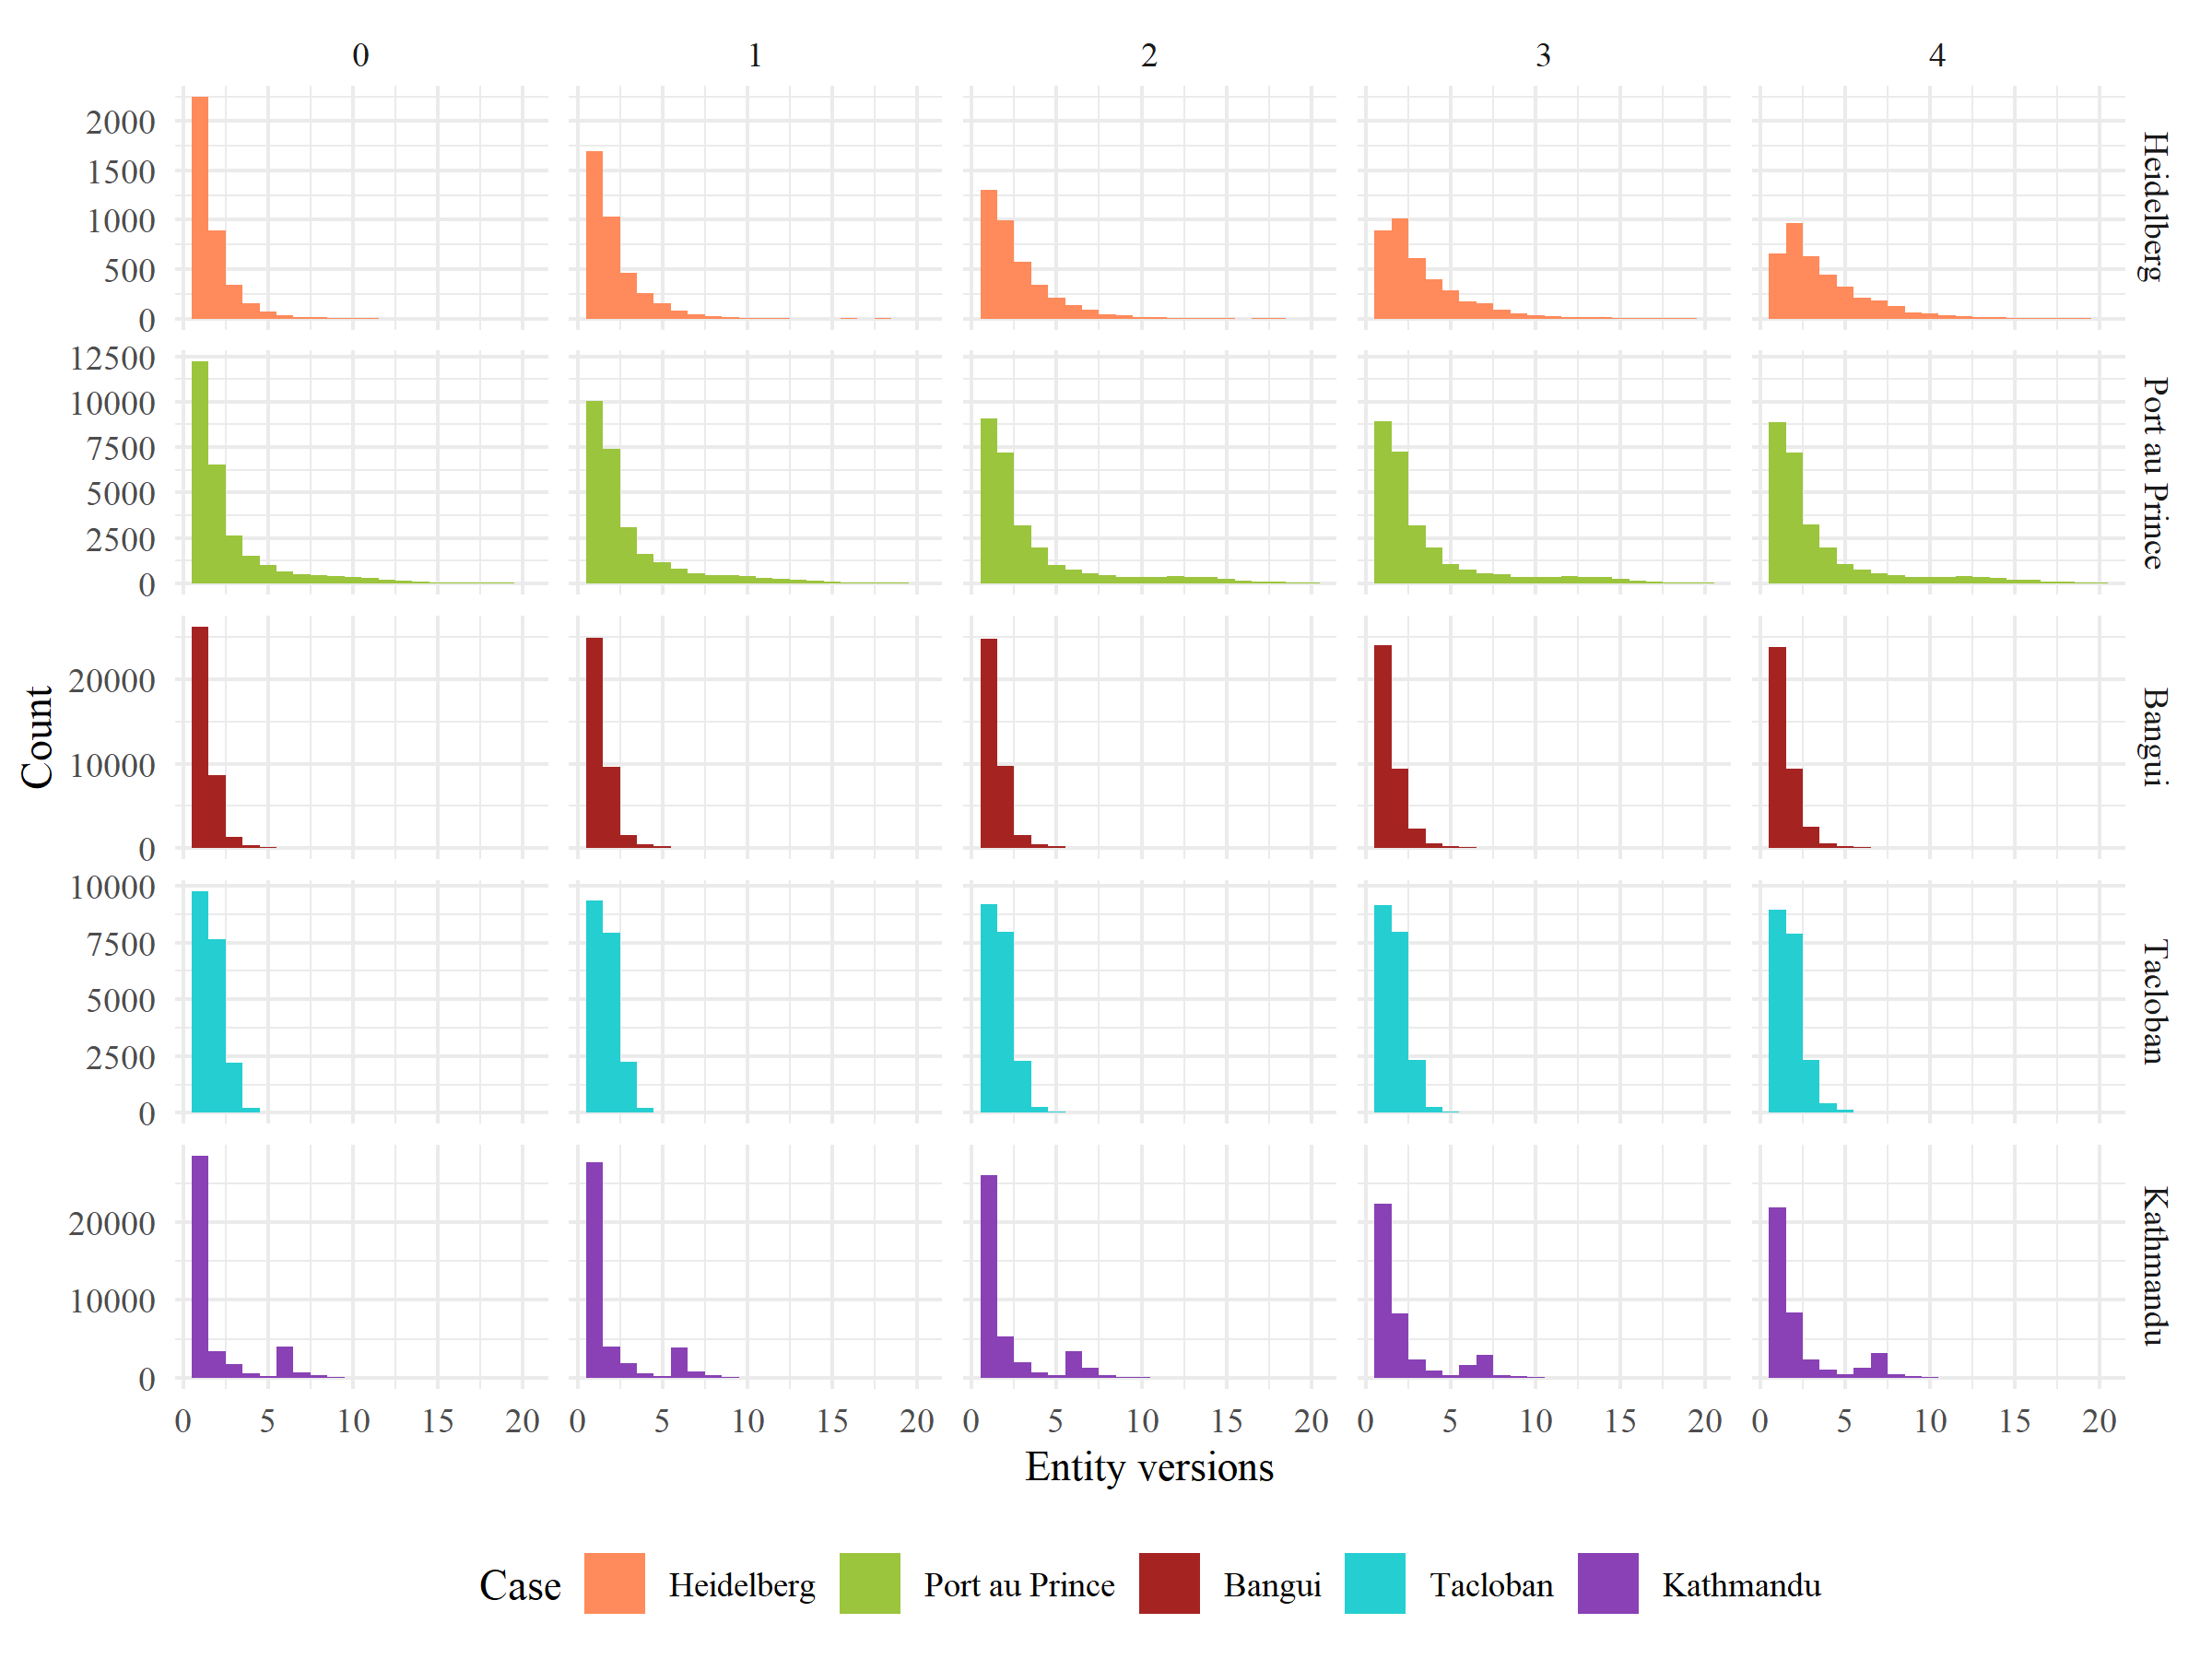
\includegraphics[width = \textwidth]{Images/facetmaint.png} %this tells latex what graphics to include. 
    \caption[Distribution of maintenance frequency for features created during each case study.]{Distribution of maintenance frequency for features created during each case study, from 1-4 years (cumulatively) since the end of each campaign.} % this prints the caption below the figure
    \label{fig:dist} % this internally labels the figure for future referencing.
\end{figure}
%%%%%%%%%%%%%%%%%%%%%%%%%% 

In Figure \ref{fig:dist} I consider data maintenance efforts by looking at the distribution in the maintenance frequency over time of all features that were created during each campaign. The x-axis of this figure is broken down by cumulative number of years since the end of the mapping campaign, and the y-axis is broken down by case study. In the first year after each mapping campaign, I see that the majority of features in all case studies have never been maintained. Changes in the distribution of maintenance frequency are the most noticeable in the Heidelberg reference case, where the passing of time leads to a distribution that is less positively skewed, and towards higher frequency of maintenance in features. After four years, many features have been maintained more than once, with the majority of features classified within the \textit{moderate} category (3-10 versions). Conversely, across all humanitarian cases, I see that the majority of features have still not been maintained after four years has passed. However, as is also reflected in Figure \ref{fig:tot}, the data from the Port au Prince and Kathmandu campaigns has been more frequently maintained than the other humanitarian cases. 

Figures \ref{fig:types} and \ref{fig:feats} illustrate the maintenance frequency distribution for features from each case study after four years have passed since the end of the mapping campaign. Figure \ref{fig:types} is disaggregated to show differences between node and way data types, and Figure \ref{fig:feats} is disaggregated to show differences between features that are tagged with the \texttt{building}, \texttt{highway}, and all other tags. In Figure \ref{fig:types}, I see that nodes and ways follow roughly the same distribution of maintenance frequency across case studies. I see similar results in Figure \ref{fig:feats}. Interestingly, however, it appears as though nodes have been relatively well-maintained in the Port au Prince case study. In Kathmandu, the majority of the \textit{other} features have been maintained at least once. Across all cases, I see that buildings are the most poorly maintained feature. 

%%%%%%%%%%%%%%%%%%%%%%%%%% Distribution of maintenance
\begin{figure} % opens the figure environment. the '[H]' forces the image to be Here
    \centering % puts the image in the horizontal centre of the page
    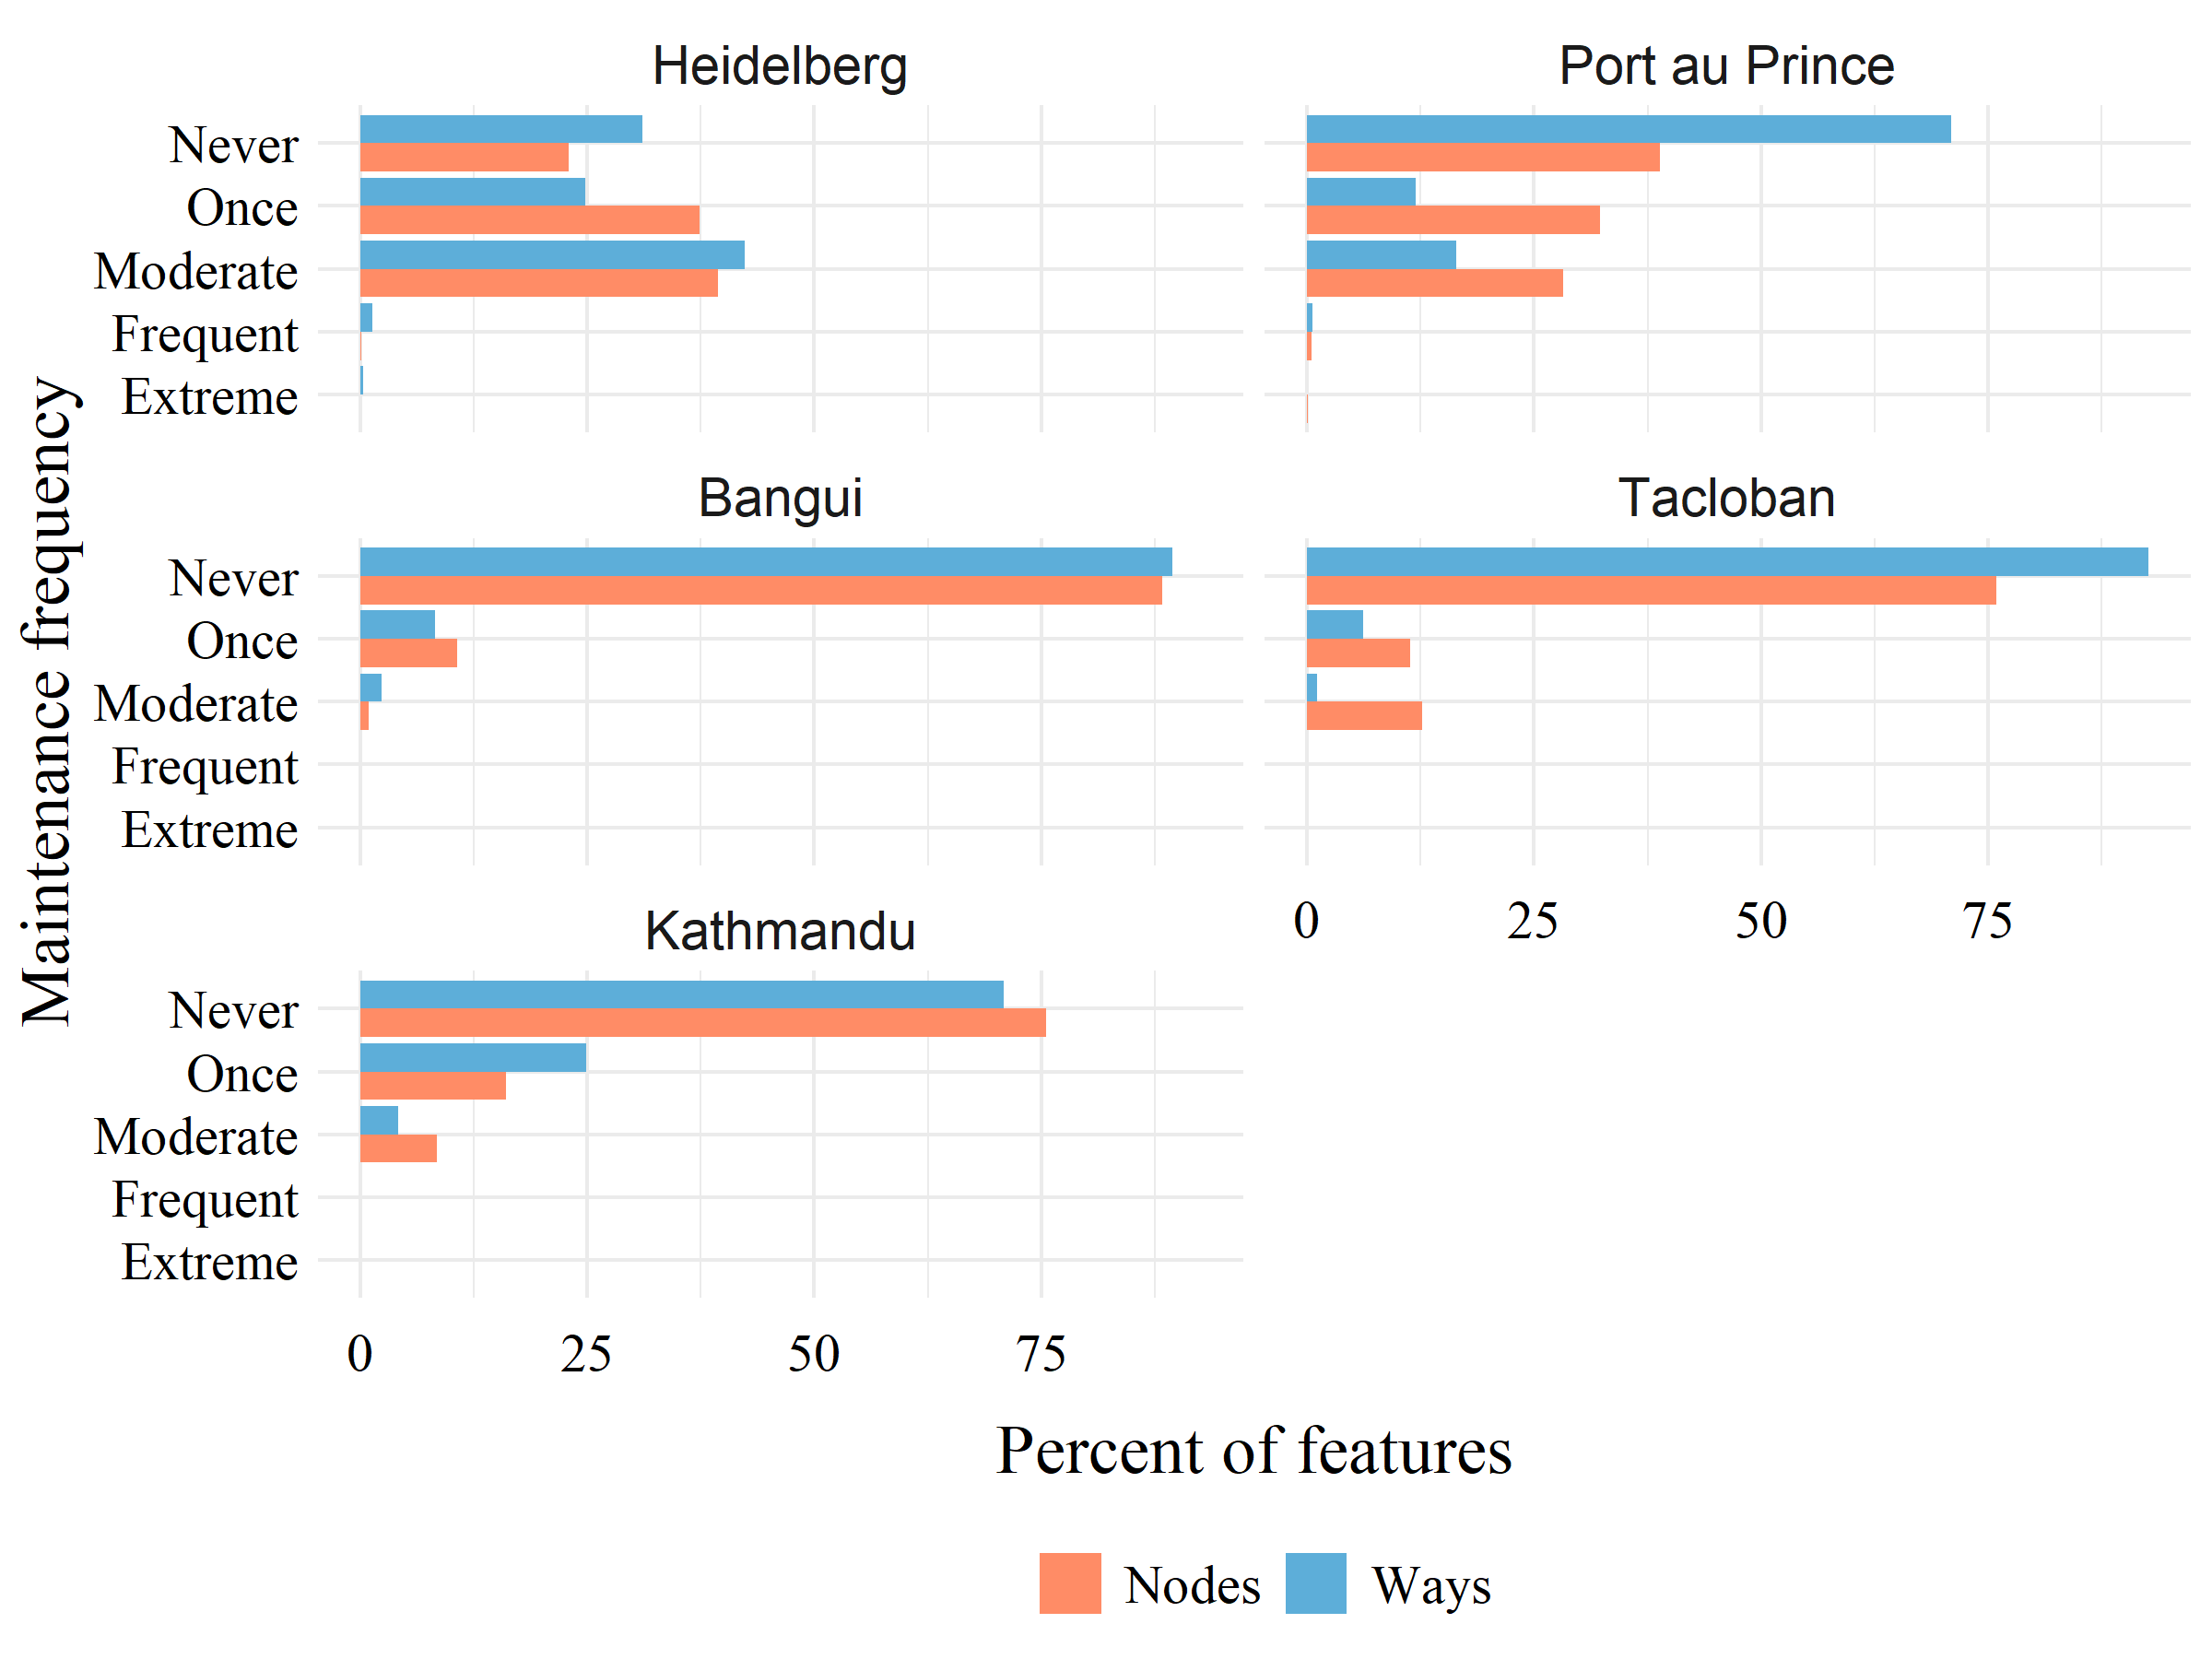
\includegraphics[width = \textwidth]{Images/typesmaint.png} %this tells latex what graphics to include. 
    \caption{Maintenance frequency of nodes and ways for each case study, four years following the end of each mapping campaign.} % this prints the caption below the figure
    \label{fig:types} % this internally labels the figure for future referencing.
\end{figure}
%%%%%%%%%%%%%%%%%%%%%%%%%% 

%%%%%%%%%%%%%%%%%%%%%%%%%% Distribution of maintenance
\begin{figure} % opens the figure environment. the '[H]' forces the image to be Here
    \centering % puts the image in the horizontal centre of the page
    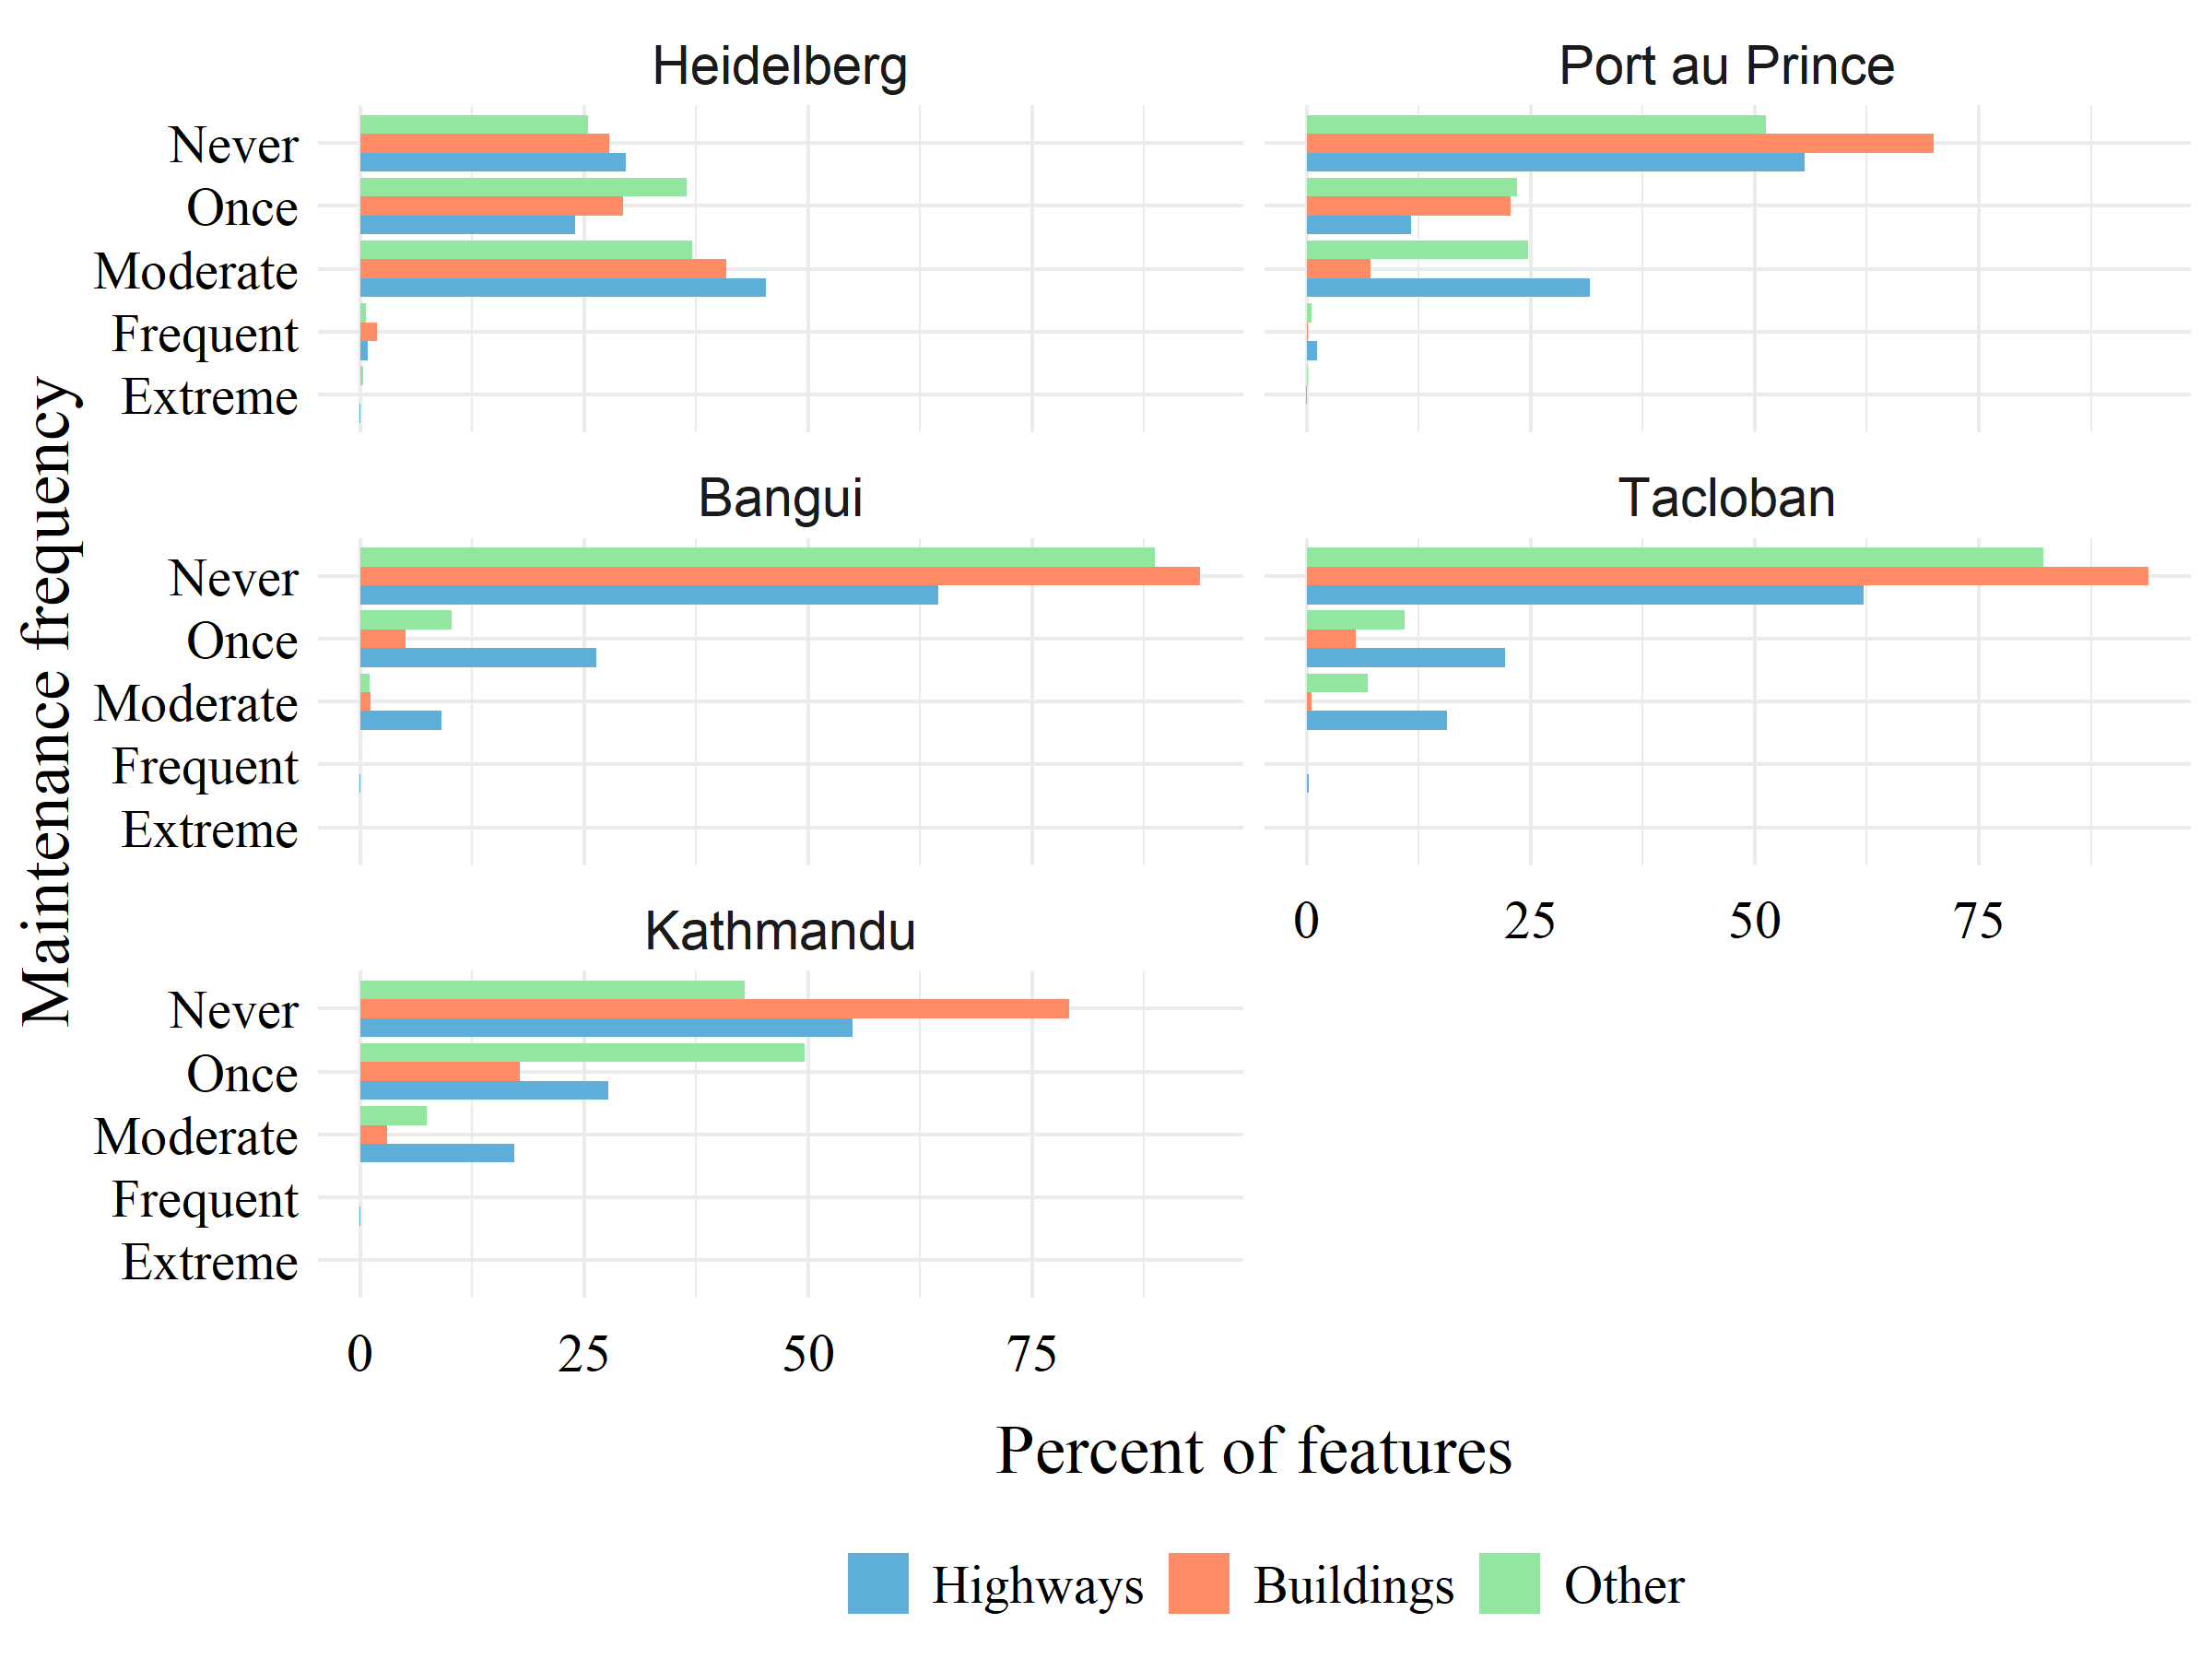
\includegraphics[width = \textwidth]{Images/featmaint.png} %this tells latex what graphics to include. 
    \caption[Maintenance frequency of features with \texttt{building}, \texttt{highway}, and all other tags for each case study.]{Maintenance frequency of features with \texttt{building}, \texttt{highway}, and all other tags for each case study; four years following the end of each mapping campaign.} % this prints the caption below the figure
    \label{fig:feats} % this internally labels the figure for future referencing.
\end{figure}
%%%%%%%%%%%%%%%%%%%%%%%%%%


\chapter{Discussion}
\label{chapterlabel6}

In this chapter we consider the results of our analysis with respect to our research question and objectives. We interpret these findings with respect to the existing body of literature that was discussed in previous chapter. We discuss the limitations of this research approach and point to potential directions for future work. 

\section{Implications for research objectives}

\noindent\textbf{Objective 1: Evaluate the characteristics of data production during the selected humanitarian mapping activations and compare against the selected reference case.} 

Our results show distinct differences between the humanitarian mapping activations and the Heidelberg reference. It is immediately apparent that the daily volume of data created reaches much higher levels during the humanitarian activations than in Heidelberg. For example, all humanitarian cases have at least one day where over 2000 features were created, while Heidelberg's maximum is only little over 100 contributions in a single day. Mapping efforts in Kathmandu, Port au Prince, and Tacloban also attracted large volumes of contributors on some days (reaching over 150 unique contributors in a single day in Kathmandu, for example), while efforts in Bangui and Heidelberg had less than 10 unique contributors each day. 

The event/mission classification scheme proposed by \textcite{dittus_mass_2017} offers a useful framework for considering data production in humanitarian mapping activations. The early peaks for the event-style activations (Port au Prince, Tacloban, and Kathmandu) shown in Figure \ref{fig:time} clearly demonstrate the dramatic burstiness that occurs when mapping is done urgently in response to an immediate natural disaster. We see that the urgency of these events leads to a rapid and significant decay in contribution volume as time passes. As shown in Figure \ref{fig:scatter}, this decay in contribution volume is correlated with a decay in contributor numbers (as is intuitive). This pattern in mapping activity from event style activations echoes the findings from \textcite[p. 1294]{dittus_mass_2017}.

While both Heidelberg and Bangui are classified as mission-style activations, Figures \ref{fig:time} and \ref{fig:scatter} show notable differences in the dynamics of how data is produced over time. Figure \ref{fig:time} shows that the volume of entities created over time in Heidelberg remains relatively stable, while mapping in Bangui has significant peaks throughout the duration of the activation. It is likely that some of these peaks are the result of data imports. This hypothesis is supported by Figure \ref{fig:scatter}, where we see the relatively weak relationship between the number of daily contributors and the daily volume of contributed data, as some days have over 1000 entities produced by fewer than four contributors. As is described in Chapter \ref{chapterlabel5}, data imports from UNICEF have been documented from this activation. While past works, such as \textcite{ahmouda_analyzing_2018}, aim to remove data imports from their analysis, we consider this to be an important part of the data production landscape that should be considered. Despite these differences, we can see that the mission-style of humanitarian mapping (as represented by the Bangui case study) is more similar to what we would consider as standard practices of OpenStreetMap data production (as represented by the Heidelberg case study) than event-style activations.

A review of the commonly-occurring tags keys shows how features such as buildings and roads are common across all case studies. This is not an unexpected finding, as these tags are among the most frequently used in all of OSM. The TagInfo\footnote{\url{https://taginfo.openstreetmap.org/}} website indicates that 58\% of all ways are tagged with \textit{building} and 24\% of all ways are tagged with \textit{highway}. Table \ref{tab:tags} also shows the different ways that tags are used to label OSM entities, across both our humanitarian and reference cases. Some tags, such as \textit{building} and \textit{highway}, correspond to geographic entities that indicate what the OSM entity is representing. Other tags, such as \textit{source} and \textit{created_by} indicate characteristics of how the data was produced. Our review of the commonly-used \textit{source} tags in Table \ref{tab:sources} shows that many of the entities from our humanitarian cases were produced from satellite sources, indicating that many contributors were remote. The prevalence of remote contributors during humanitarian mapping activations is well-understood within the literature \parencite{dittus_mass_2017, eckle_quality_2015}. While very few of the entities from Heidelberg were tagged with a \textit{source}, we do not see the presence of any satellite sources, indicating that this data was more likely to be produced by local mappers. Interestingly, we also see the presence of disaster-related tags in the humanitarian cases, such as \textit{typhoon:damage, idp:camp_site}, and \textit{damage:event}. These disaster tags correspond to temporary attributes, suggesting that they will likely need to be removed or updated in the future. \\

\noindent\textbf{Objective 2: Empirically assess the extent to which data is maintained after each humanitarian mapping activation.}

In this work we present multiple approaches for quantifying data maintenance following each of our case study mapping activations in OSM. We consider maintenance from both a binary and categorical perspective, acknowledging that a given entity may be updated (ie. maintained) any number of times and thus different degrees of data maintenance can take place. 

Figures \ref{fig:tot}, \ref{fig:dist}, and \ref{fig:types} all show how the data from our Heidelberg reference has been maintained to a significantly greater extent than the data from our humanitarian case studies. Heidelberg is the only case study where over 50\% of the entities have been updated or deleted at least once since being created. This finding is in line with our hypothesis, as we have selected Heidelberg as a reference due to its highly engaged community of mappers and comparatively complete and accurate data. While we are careful not to generalize our findings beyond the case studies that we have selected, this result suggests that OSM data produced from humanitarian mapping efforts may be less maintained than other subsets of the database. Greater effort may thus be needed in ensuring that the data produced in response to humanitarian need is maintained in OSM in the years following the activation. 

These findings may have implications for our understanding of the temporal accuracy of OSM data in areas that have been subjects of humanitarian mapping activations. In Chapter \ref{chapterlabel2}, we discussed how data maintenance can be considered as the process by which OSM data is kept up-to-date. 

Our findings suggest a potential problem with the current mechanisms of data production during humanitarian mapping activations. As is shown by our case studies, these activations may produce an incredibly large volume of data over short periods of time (eg. nearly 40,000 nodes and ways produced in Kathmandu alone in less than one year). While there is no denying that this data is immediately useful in the wake of a disaster, for example, it also presents a challenge in that there is now more data that can potentially be out of date in the future if it is not well maintained. Ideally the data produced during a humanitarian activation is of lasting value to the local community, so care should be taken in how it is maintained.

While stakeholders in the humanitarian mapping community, such as HOT, are well-aware of the importance of engaging local communities of contributors in data production, the justification for doing so is not necessarily framed in terms of data maintenance. 

\noindent\textbf{Objective 3: Consider factors of data production that may have an impact on levels of data maintenance.}

It can logically be assumed that low levels of data maintenance are the result of one of two things: 1) there is no need for maintenance as the underlying geography of a given region remains the same, or 2) there is no one with the necessary skills or motivation to do the work involved in maintaining data. 

\noindent\textbf{Objective 4: Distill key findings into recommendations for the humanitarian mapping community.}

\section{Limitations and directions for future work}

The novelty of our research aims posed a challenge in that we were unable to rely on an established analytical workflow for our data processing efforts. The existing literature does not offer an established analytical framework for investigating characteristics of data production and data maintenance during humanitarian mapping activations. We deemed commonly-used spatio-temporal data mining techniques; such as clustering, pattern recognition, and predictive learning; to be inappropriate for our dataset and research aims. 

We note that, as indicated by the approach taken in \textcite{mooney_characteristics_2012}, a higher number of versions for a given entity may not correspond to our definition of maintenance. Many versions may also correspond to cases where the entity needs to be revised, perhaps due to errors made in the initial mapping efforts or to disagreements in how the entity should best be mapped. In the case of humanitarian mapping, the \textit{validation} process also requires that features be reviewed, which may result in new, corrected versions for a given entity (which is, again, not necessarily maintenance). 

Given the little past work in this domain, it is difficult to know how much data maintenance is necessary in a given area. Theoretically, we understand that data only needs to be maintained if the associated geographic phenomena have changed in some way. We assume that it is incredibly unlikely for all geographic phenomena in an area to remain the same over a long period of time, so we understand that, given the passing of time, some data maintenance will always be necessary. However, given that we have no ‘ground-truth’ for how much change has occurred in a given area, it is challenging to know whether or not an apparently lack of data maintenance is a problem or not.  


\chapter{Conclusion}
\label{chapterlabel7}

This research employs a comparative case study approach to investigate data production and maintenance in humanitarian mapping campaigns. This work responds to the need to more rigorously consider dimensions of temporal data quality in OSM, particularly within humanitarian mapping contexts. We focused specifically on humanitarian campaigns in Port au Prince, Bangui, Tacloban, and Kathmandu; and compare against mapping in Heidelberg as a reference. The recently developed OSHDB API was applied to efficiently process and filter large volumes of historical OSM data. In addition to the key results summarized below, this research builds off of \textcite{quattrone_work_2017} and offers a methodological approach for empirically assessing data maintenance in OSM.  

Following the framework set out by \textcite{dittus_mass_2017}, we classified Bangui and Heidelberg as mission-style campaigns; and Tacloban, Kathmandu, and Port au Prince as event-style campaigns. Our humanitarian case studies differed from our Heidelberg reference in both the overall and daily volume of new contributions to OSM, with the humanitarian campaigns showing significantly more data added over shorter time frames. 

Our results also show that the data produced during our selected humanitarian campaigns has been poorly maintained over time when compared against the maintenance levels seen in Heidelberg. Across all humanitarian case studies, the majority of data produced during the mapping campaign has not been modified or deleted after four years. This finding suggests that the OSM data in these areas is at a greater risk of becoming out of date. Thus, the humanitarian mapping community may need to consider developing formal mechanisms or incentives for ensuring that the data produced during mapping campaigns is maintained over time, allowing for it to be a lasting resource for the affected communities. 




%%%%%%%%%%%%%%%%%%%%%%%%%%%%%%%%%%
% BIBLIOGRAPHY AND APPENDICES
%%%%%%%%%%%%%%%%%%%%%%%%%%%%%%%%%%
\phantomsection
\addcontentsline{toc}{chapter}{Bibliography}
\printbibliography
%\addcontentsline{toc}{chapter}{Appendices}

% The \appendix command resets the chapter counter, and changes the chapter numbering scheme to capital letters.
%\chapter{Appendices}
\appendix
\chapter{An Appendix About Stuff}
\label{appendixlabel1}
(stuff)

\chapter{Another Appendix About Things}
\label{appendixlabel2}
(things)

\chapter{Colophon}
\label{appendixlabel3}
\textit{This is a description of the tools you used to make your thesis. It helps people make future documents, reminds you, and looks good.}

\textit{(example)} This document was set in the Times Roman typeface using \LaTeX\ and Bib\TeX , composed with a text editor. 
 % description of document, e.g. type faces, TeX used, TeXmaker, packages and things used for figures. Like a computational details section.
% e.g. http://tex.stackexchange.com/questions/63468/what-is-best-way-to-mention-that-a-document-has-been-typeset-with-tex#63503

% Side note:
%http://tex.stackexchange.com/questions/1319/showcase-of-beautiful-typography-done-in-tex-friends



% All done. \o/
\end{document}
